\chapter{Auswertung}
\label{chap:Auswertung}
In diesem Kapitel sollen die im Experiment ermittelten Messdaten ausgewertet werden. Bereits bei einer Kalibrationsmessreihe mit Argon konnten aufgrund einer Fehlfunktion der Elektronenkanone keine vollständigen Wirkungsquerschnitte aufgenommen werden. Die Zahl der Elektronen, die für die Berechnung des Wirkungsquerschnittes benötigt werden, kann, gerade bei geringeren Elektronenenergien, nicht ausreichend genau eingestellt werden, sodass keine Messung der Ladung möglich ist. Nach einem Austausch der Heizkathode können die Messungen fortgesetzt werden. 

Aus diesem Grund kann nur eine qualitative bzw. relative Auswertung einer Kalibrationsmessung mit Argon sowie eines Restgasspektrums durchgeführt werden und es können keine absoluten Werte für die Ionisationsquerschnitte berechnet werden. Ein besonders kleiner Extraktionsstrom der Kanone bei niedriger Elektronenenergie macht eine Messung des Elektronenstroms zu ungenau. Die Bestimmung der Ionisierungsquerschnitte ist nicht möglich, da die Elektronenzahl direkt in die Formel eingeht, es können jedoch qualitative Aussagen über die relativen Häufigkeiten der Ionen getroffen werden, welche proportional zum Ionisierungsquerschnitt sind. Anschließend folgt eine Simulation des Massenspektrometers der Ionenoptik in Kapitel \ref{chap:Simulation}, mit der die Genauigkeit des Massenspektrometers überprüft werden kann.

\section{Kalibrationsmessung mit Argon}
Um die Anlage mit einem bereits gut untersuchten Gas zu testen, wurde eine Testreihe mit Argon durchgeführt. Die Auswertung der Messdaten erfolgt über einen digitalen Vielkanalanalysator (MCA), der auf einem Computer Histogramme der aus der Flugzeit generierten Pulshöhen erstellt. Der MCA hat 4096 diskrete Kanäle, welche den Zeitbereich von Null bis zur maximalen Zeit des TPHC abdecken. Diese werden dann mit den \textsc{python}-Bibliotheken \textsc{matplotlib}, \textsc{SciPy} und \textsc{numpy} weiter ausgewertet und dargestellt. 
\begin{figure}
    \hspace{-1.1cm}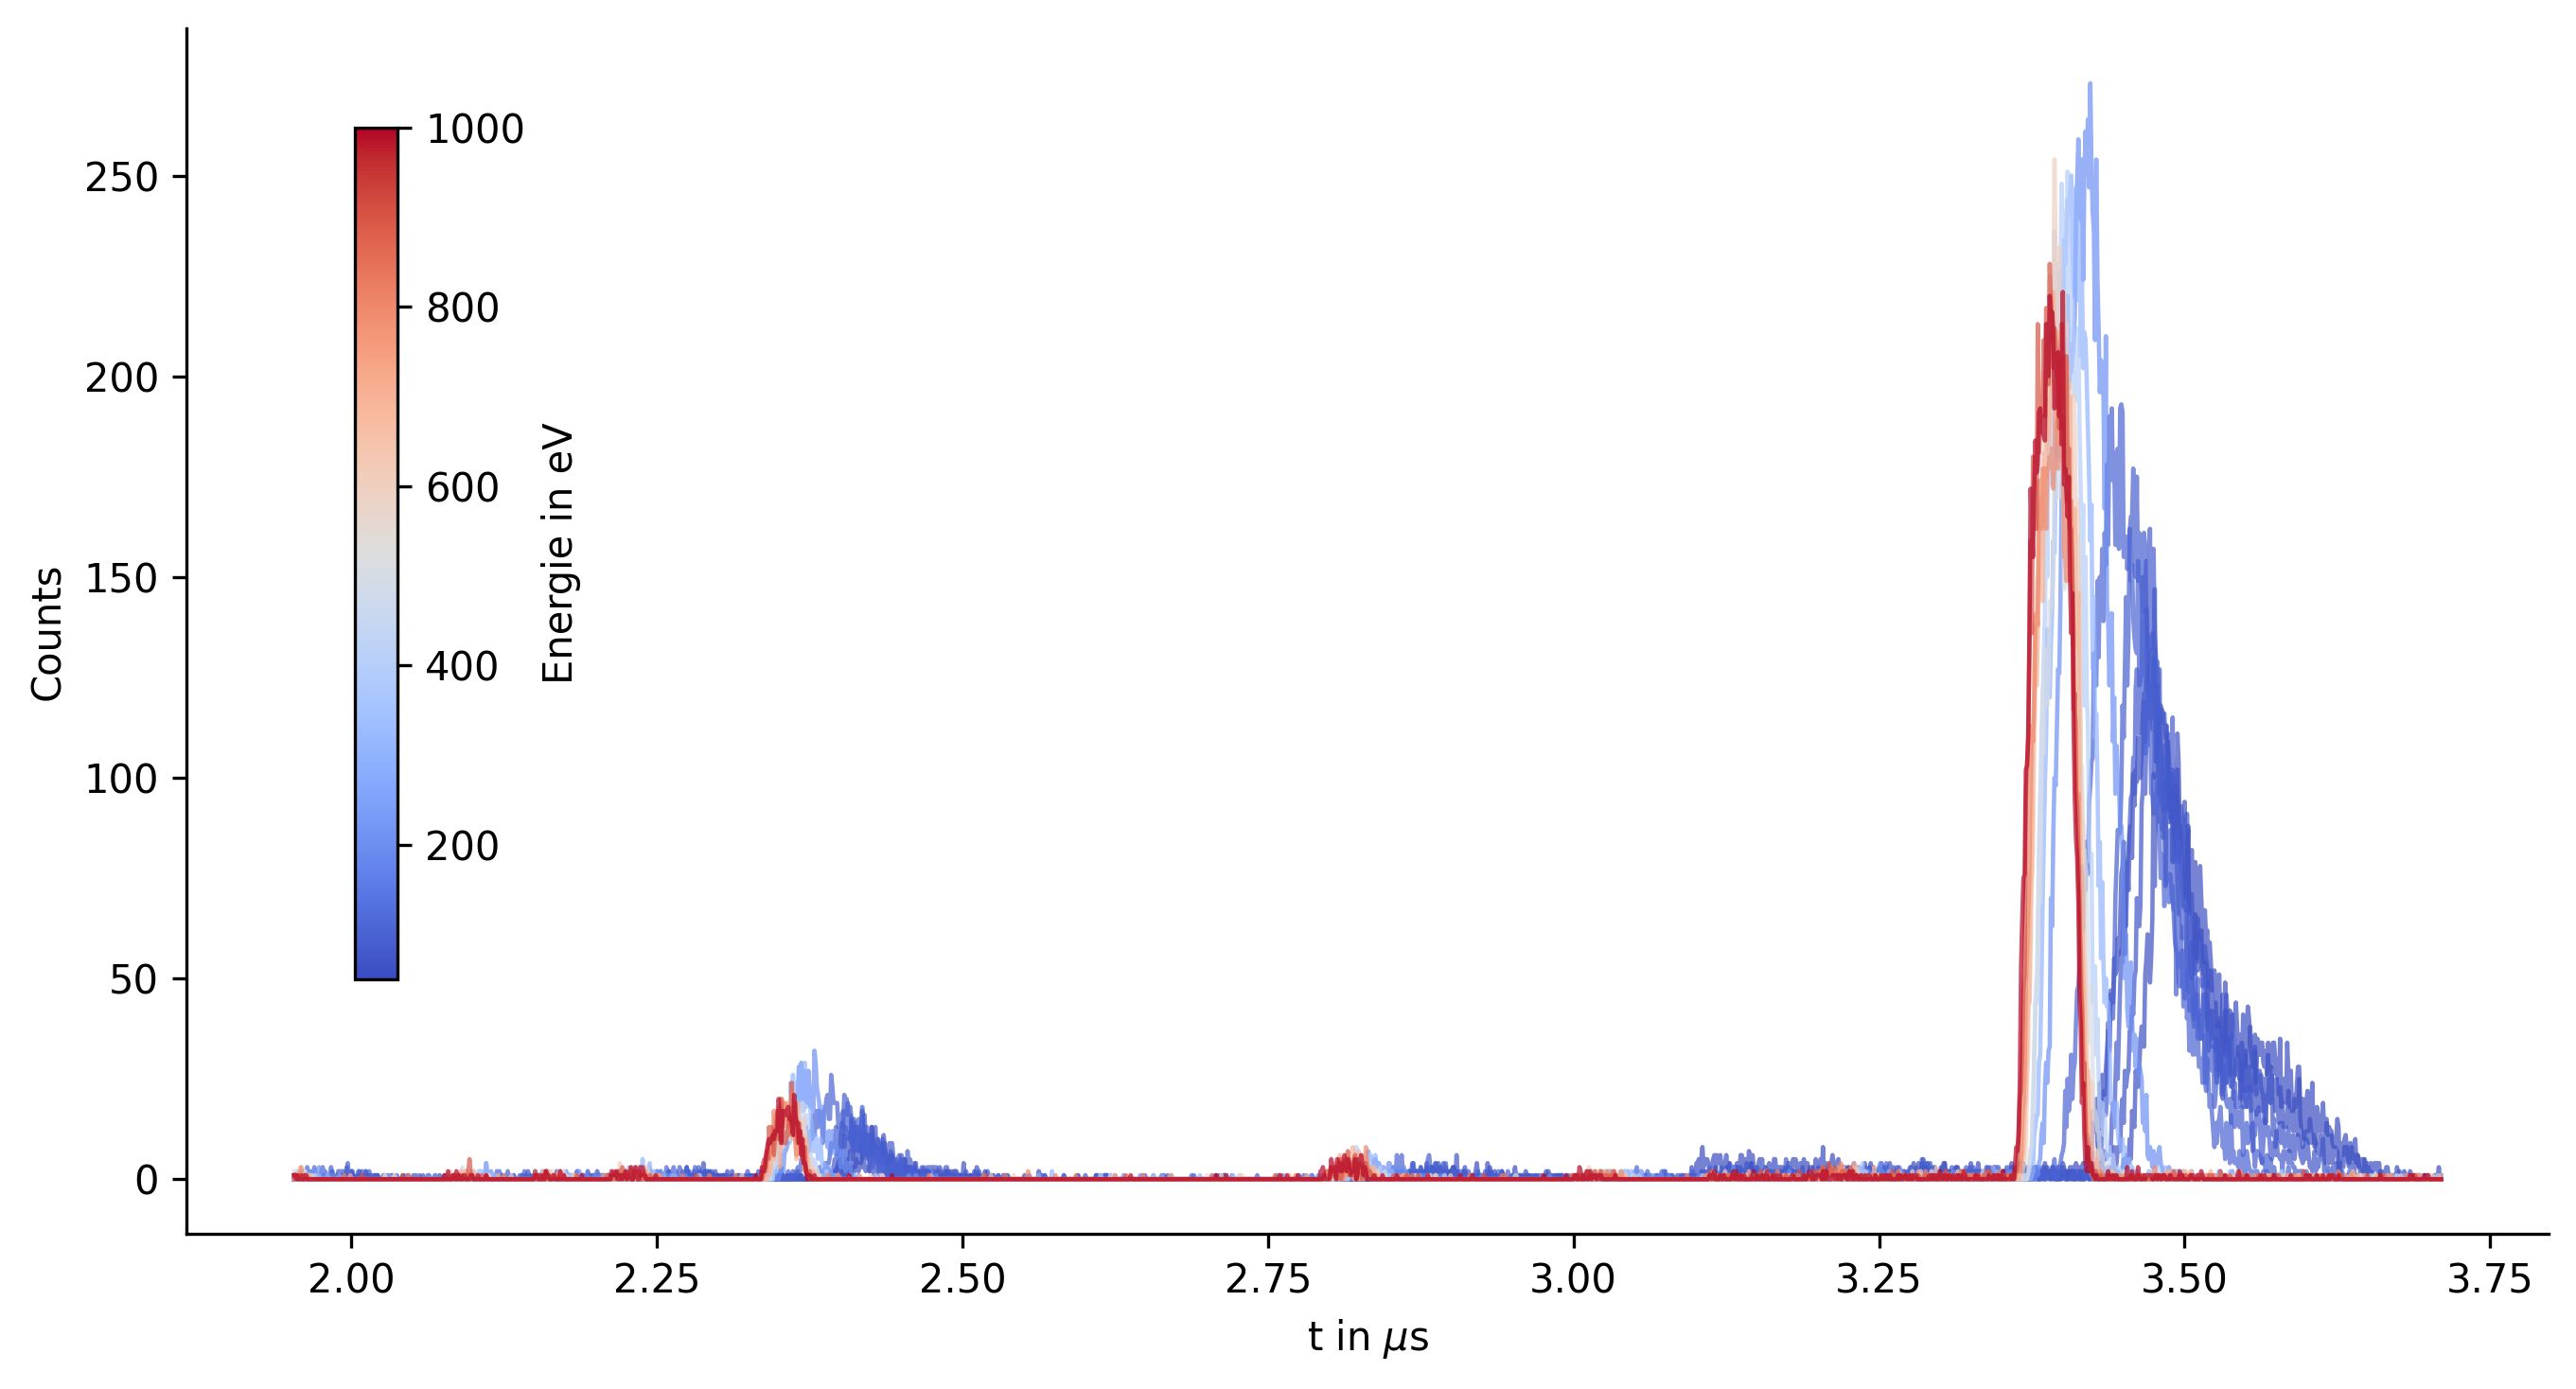
\includegraphics[width=1.08\textwidth]{Ar50-1000eV.png}
    \caption[Flugzeitspektrum von Argon bei Elektronenenergien von 50 bis 1000 eV]{Flugzeitspektrum von Argon bei Elektronenenergien von 50 bis 1000 eV. Die Messungen sind jeweils über 60 Sekunden entstanden.}
    \label{fig:ar}
\end{figure}
Abbildung \ref{fig:ar} zeigt unskalierte Flugzeitspektren von Argon bei Elektronenenergien von 50 bis 1000 eV. Es ist zu erkennen, dass die Peaks mit steigender Elektronenenergie schärfer werden und es einen Zusammenhang zwischen der Elektronenenergie und der Flugzeit gibt, der im Folgenden genauer untersucht wird. Dass die Peaks schärfer werden, ist unter anderem darauf zurückzuführen, dass die Elektronenkanone bei höheren Energien einen schärferen Strahl erzeugt. Die thermische Bewegung der Elektronen hat wenig Einfluss gegenüber der deutlich höheren kinetischen Energie. Der Entstehungsort der Ionen ist dann genauer definiert, was zu schmaleren Peaks führt.

\subsection{Zusammenhang von Flugzeit und Elektronenenergie}
Woher genau der Zusammenhang zwischen Flugzeit und Elektronenenergie kommt, kann nicht direkt aus den Daten abgeleitet werden, da ein höherer Energieübertrag auf die Gasatome nicht direkt die Flugzeit beeinflussen kann. Es kann aber vermutet werden, dass dieses Phänomen mit der verzögerten Extraktion der Ionen aus dem Kondensator zusammenhängen könnte. Genauere Untersuchungen folgen in Kapitel \ref{sec:delay_sim} im Rahmen der Simulation. Anhand der mittleren Flugzeit des größten Peaks der verschiedenen Spektren kann der Zusammenhang zwischen der Elektronenenergie und der Flugzeit untersucht werden.
Abbildung \ref{fig:tof_energy} zeigt die Flugzeit des größten Peaks in Abhängigkeit der Elektronenenergie. Es ist zu erkennen, dass die Flugzeit mit steigender Elektronenenergie $E$ sinkt. Ein Fit der Form $t(E) = -a\sqrt{E} + b$ zeigt, dass die Flugzeit proportional zu $-\sqrt{E}$ ist. $a$ und $b$ sind dabei Fitparameter, die die Steigung und den Offset des Zusammenhangs beschreiben. 

\begin{figure}
    \centering
    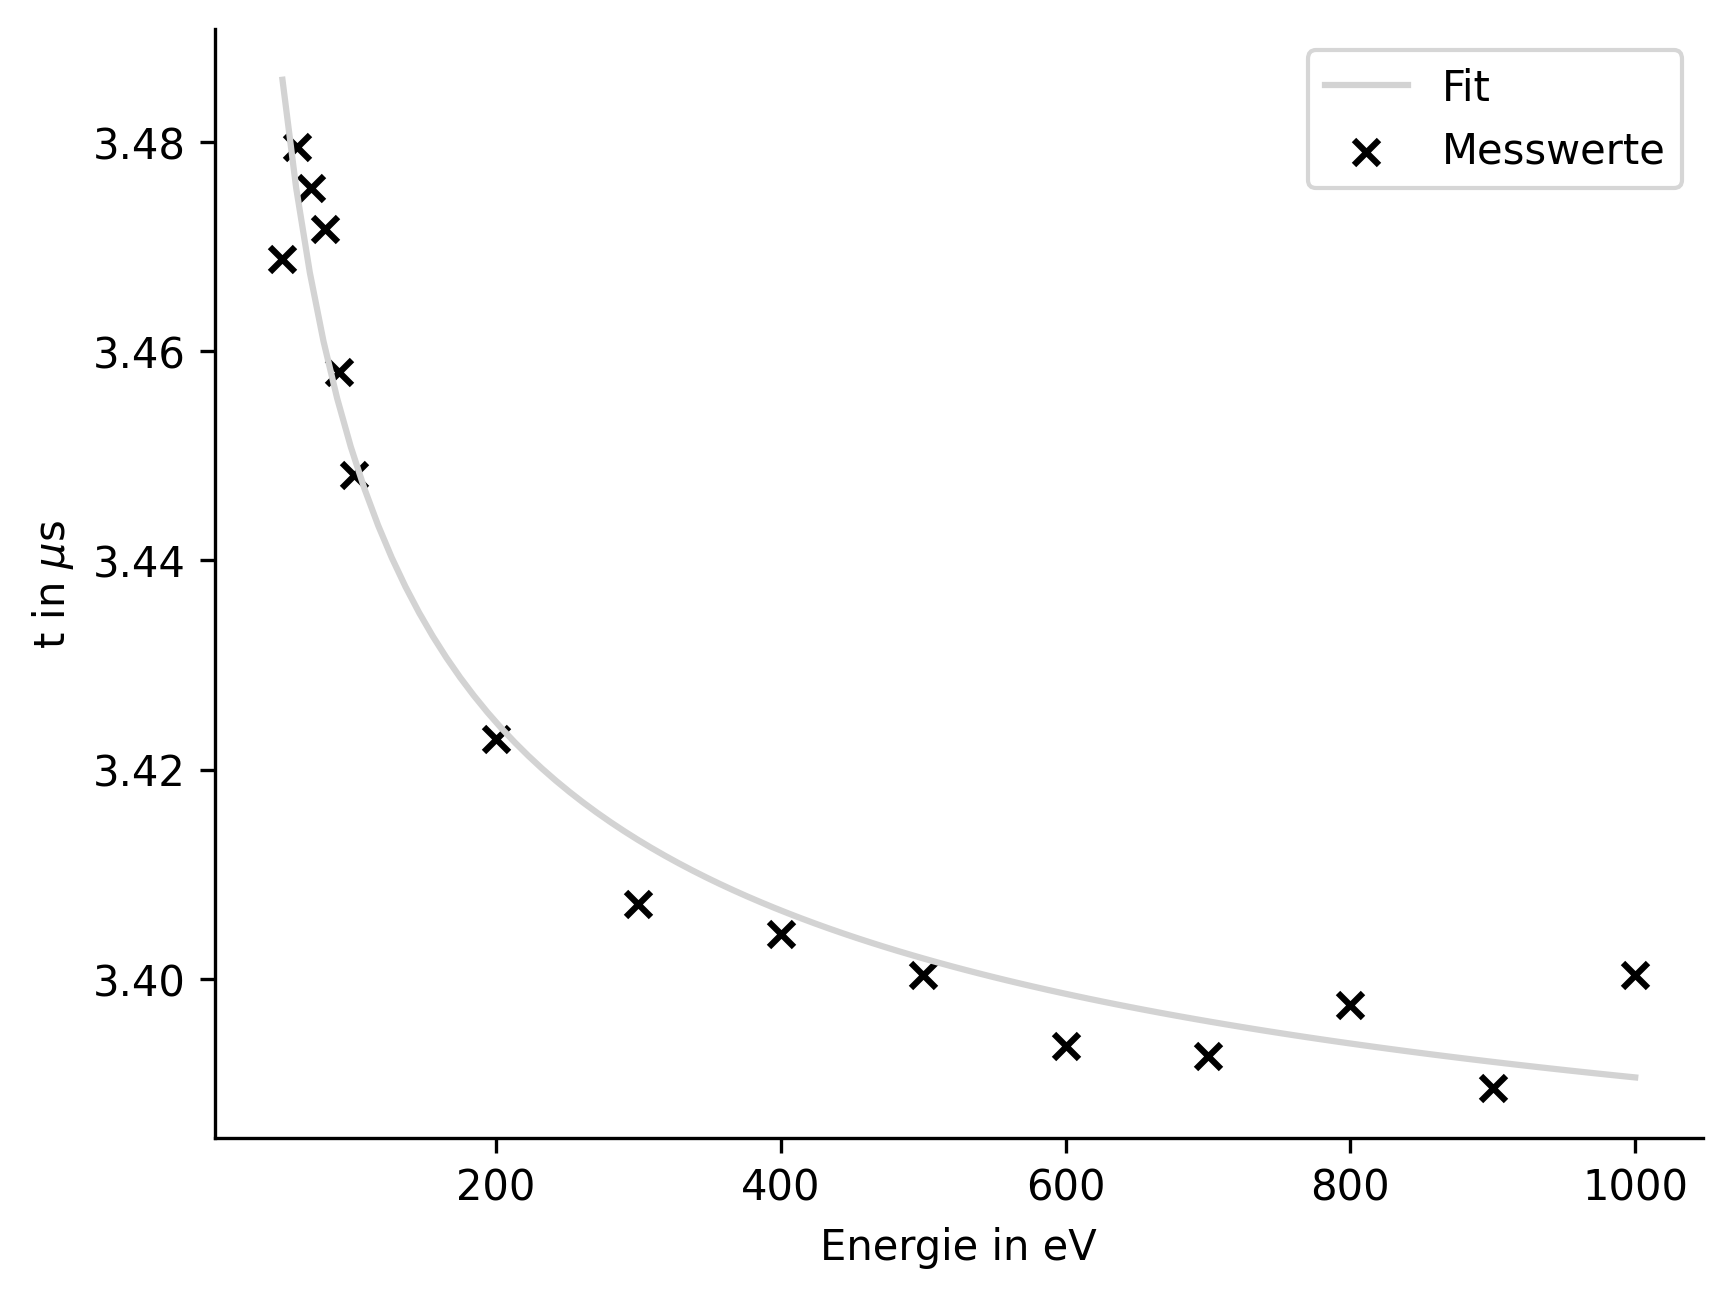
\includegraphics[width=.7\textwidth]{tof_energy.png}
    \caption[Zusammenhang zwischen TOF und Elektronenenergie]{Abbildung der Flugzeit des größten Peaks in Abhängigkeit der Elektronenenergie. Ein Fit zeigt, dass eine Funktion der Form $t(E) = -a\sqrt{E} + b$ den Zusammenhang gut beschreibt.}
    \label{fig:tof_energy}
\end{figure}

\subsection{Transformation in ein Massenspektrum}
\label{sec:transformation}
Für eine weitere Analyse muss das Flugzeitspektrum in ein Massenspektrum transformiert werden. Um das Spektrum korrekt skalieren zu können, werden die Peaks mit einem Referenzspektrum verglichen und einzelne identifiziert. Im Fall der Kalibrationsmessung mit Argon wurde ein Spektrum von Straub et al. \cite{Straub} als Vergleich verwendet, bei dem die Peaks von ein- bis vierfach geladenen Argonionen identifiziert wurden. Anhand dieser Information kann das Spektrum skaliert werden, um die Masse-zu-Ladungsverhältnisse auf der horizontalen Achse zu erhalten. Die Transformationsfunktion hat die Form $at^2+b$, wobei die Parameter über die Zuordnung des Masse-zu-Ladungsverhältnisses von mindestens drei Punkten ermittelt werden können. Diese Form beschreibt die Abhängigkeit des Masse-zu-Ladungsverhältnisses von der Flugzeit hinreichend gut, da die gesamte Flugzeit nach Gleichung \ref{eq:time} proportional zu $\sqrt{m/q}$ ist. Zusätzlich kann mit einem zweiten Parameter ein Offset eingestellt werden, der durch Einstellungen am ADC entstehen kann. 

Um einen Vergleich mehrerer Spektren zu ermöglichen, werden die Spektren zunächst normalisiert. Das bedeutet, dass die Fläche des größten Peaks $N_\text{peak}(\text{Ar}^+$) auf 1 gesetzt wird. Da sich der Ionisationsquerschnitt mit der Elektronenenergie ändert, werden die Spektren anschließend mit den Werten für $\sigma_+$ von Straub et al. gewichtet. Das wird genauer in Kaptiel \ref{sec:Analyse} erläutert.

Durch die begrenzte Zahl der Kanäle des MCA ergibt sich eine Unsicherheit 
\begin{equation}
    \Delta t_{\mathrm{MCA}} = \frac{4 \text{ \textmu{s}}}{4096} = 0.977 \text{ ns},
\end{equation} 
die sich auf eine Massenunsicherheit umrechnen lässt. Dafür muss die Fehlerfortpflanzung der Transformationsfunktion berücksichtigt werden:
\begin{equation}
    \Delta m/q = \sqrt{\left(\frac{\partial f_\mathrm{Trans}}{\partial t}\right)^2 \Delta t_{\mathrm{MCA}}^2} = 2at\Delta t_{\mathrm{MCA}}.
\end{equation}
$a$ ist dabei der erste Parameter der Transformationsfunktion $f_\mathrm{Trans}$, der bei einer Elektronenenergie von 100 eV bei einem Argonspektrum $3.02 \cdot 10^{-6}$ beträgt. Bei einer Flugzeit von 3.5 \textmu{s} beträgt dann die Unsicherheit der Masse 0.129 u/e. Das bedeutet, dass eine Masse von 40 u/e mit einer Unsicherheit von 0.129 u/e gemessen wird. Die Auflösung ist in der Realität kleiner, da die Peaks nicht unendlich schmal sind und sich über mehrere Kanäle erstrecken.

\subsection{Extraktionsverzögerung}
\label{sec:delay}
Die Verzögerung der Extraktion bei der DETOF-Methode ermöglicht schärfere Flugzeitpeaks. Für die bisherige Auswertung wurde eine tatsächliche Extraktionsverzögerung von etwa 300 ns verwendet. Das geht aus den Signalen hervor (Abbildung \ref{fig:Signal}). Besonders bei niedrigen Energien sind die Peaks sehr breit und unsymmetrisch. Eine Verdopplung der Extraktionszeit auf 600 ns macht die Peaks deutlich schärfer und verbessert so auch die darstellbare Auflösung. Abbildung \ref{fig:delay} zeigt die Flugzeitspektren von Argon bei 50 eV mit einer Extraktionsverzögerung von 300 ns und 600 ns. Eine weitere Verlängerung der Extraktionsverzögerung hat nicht denselben Effekt. Aufgrund der deutlichen Verbesserung sind folgende Spektren mit 600 ns Verzögerung aufgenommen worden.
\begin{figure}
    \centering
    \begin{subfigure}{.48\textwidth}
        \centering
        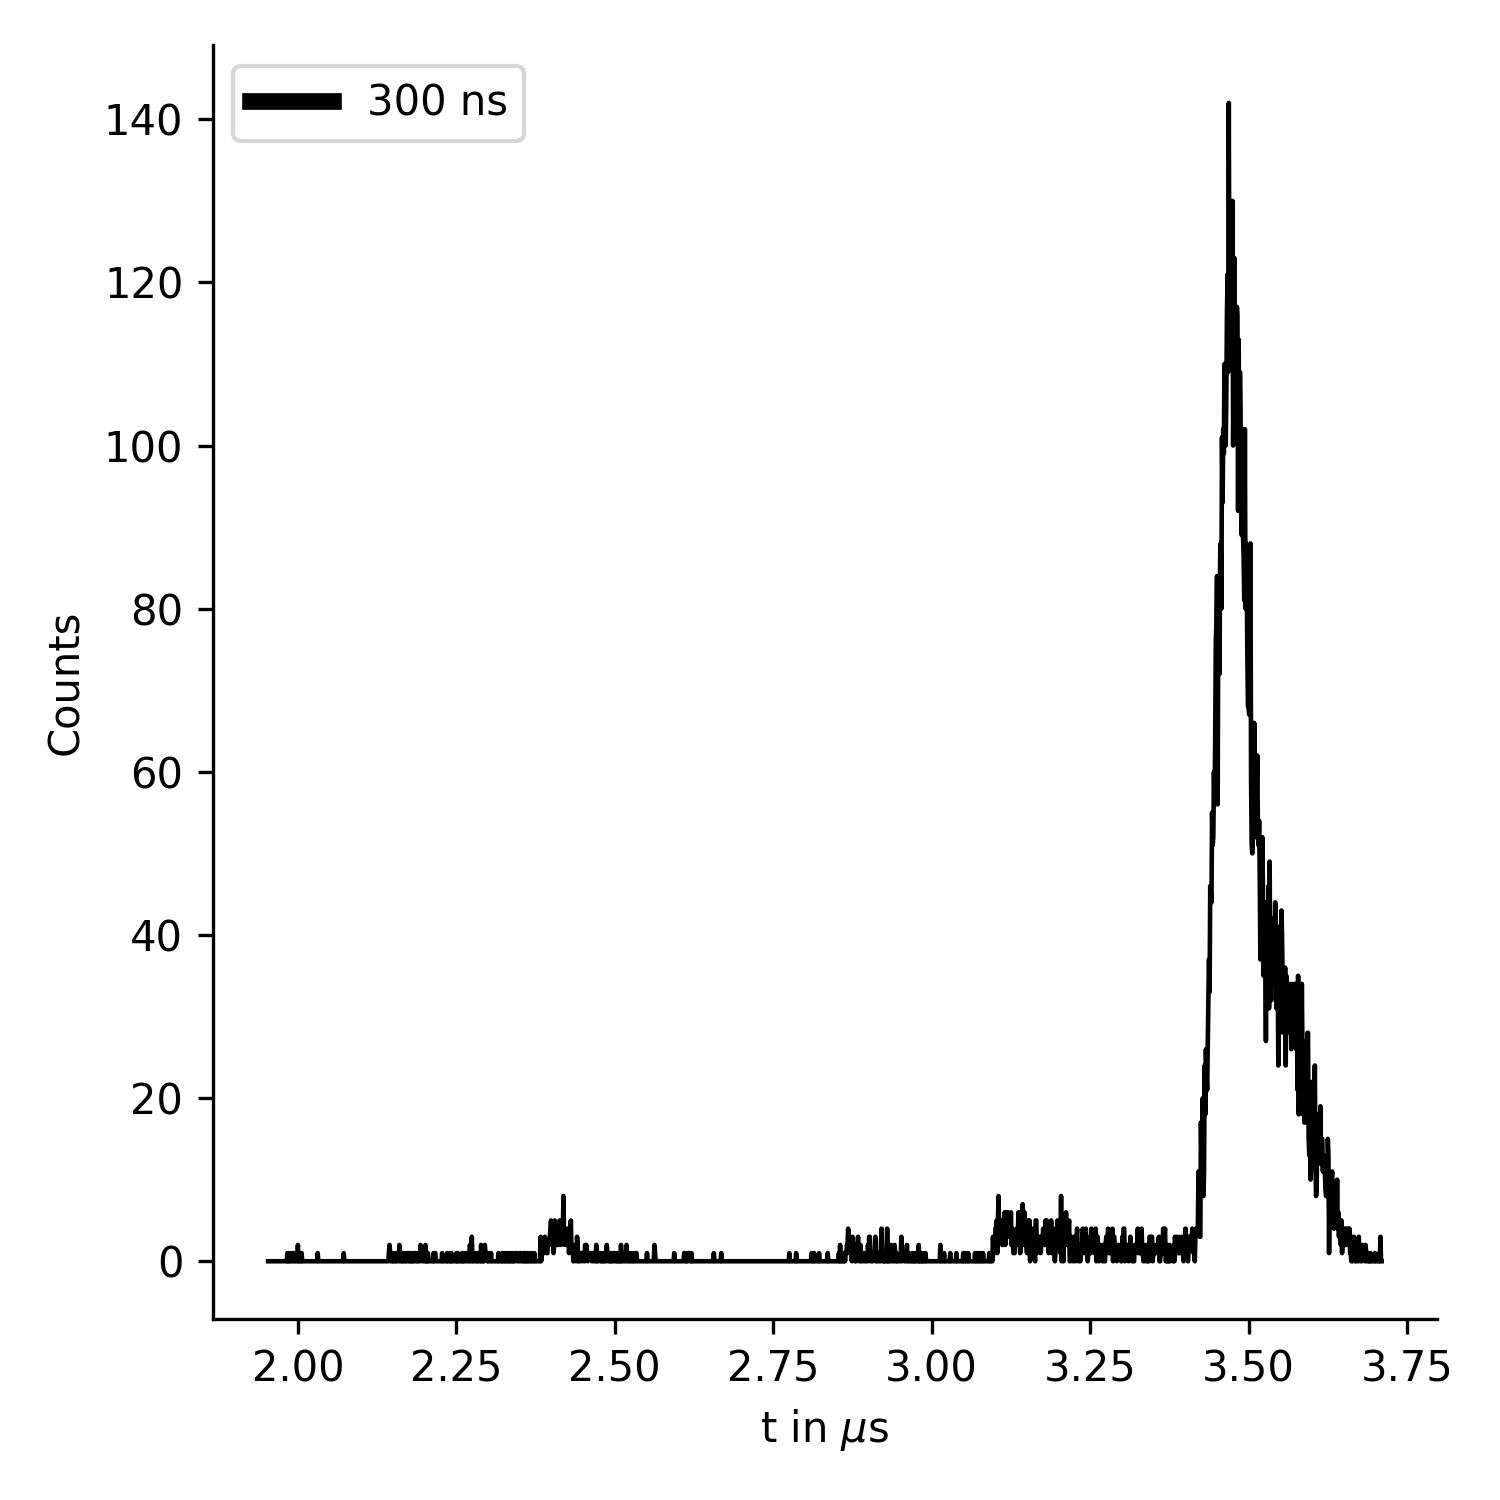
\includegraphics[width=.97\linewidth]{Ar50-300ns.png}
        \caption{Argon bei 50 eV Elektronenenergie mit 300 ns Extraktionsverzögerung}
    \end{subfigure}%
    \hfill
    \begin{subfigure}{.48\textwidth}
        \centering
        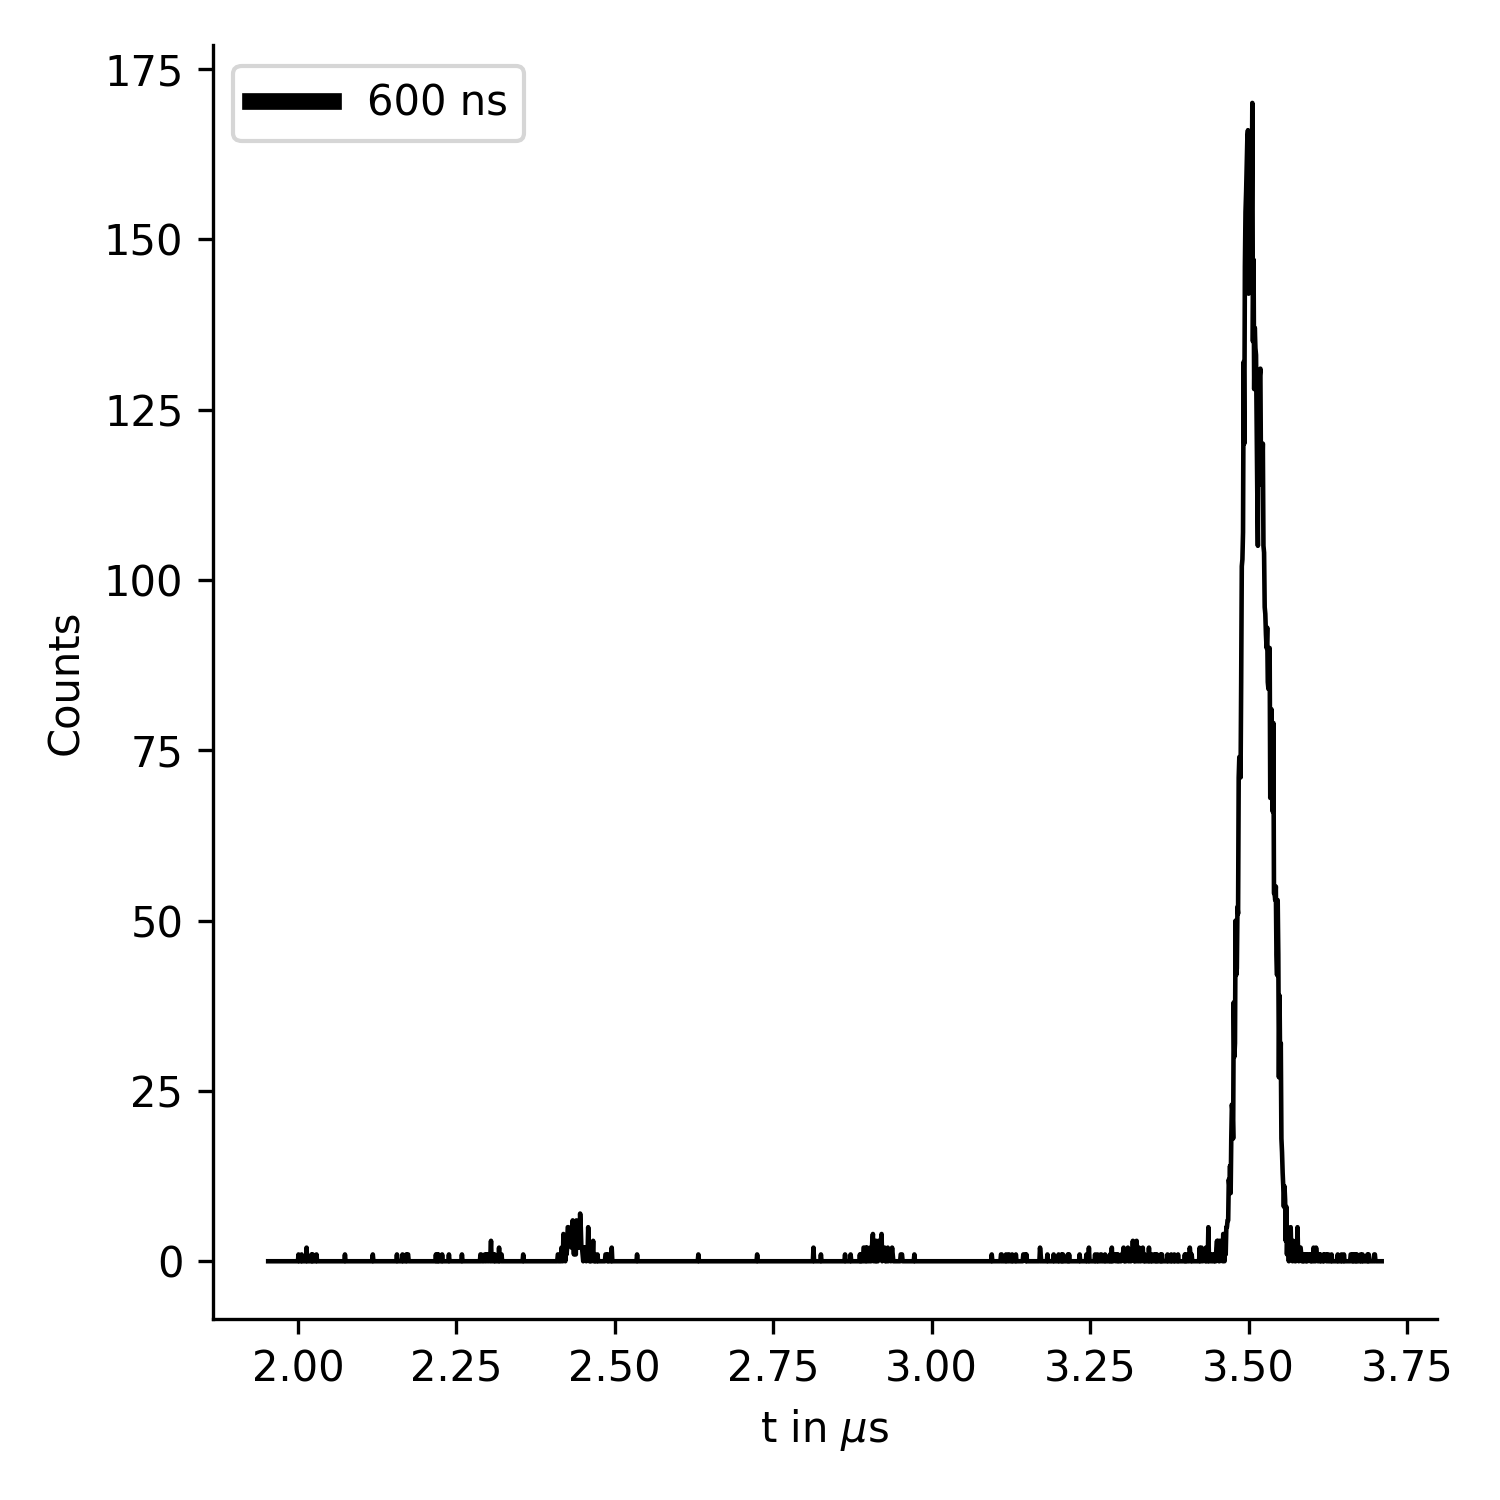
\includegraphics[width=.97\linewidth]{Ar50-600ns.png}
        \caption{Argon bei 50 eV Elektronenenergie mit 600 ns Extraktionsverzögerung}
        
    \end{subfigure}
    \caption[Einfluss der Extraktionsverzögerung auf Flugzeitspektren]{Flugzeitspektren von Argon bei 50 eV mit unterschiedlichen Extraktionsverzögerungen.}
    \label{fig:delay}
\end{figure}


\subsection{Analyse und Vergleich der Ergebnisse}
\label{sec:Analyse}
Abbildung \ref{fig:ar_scaled} zeigt ein Massenspektrum von Argon. Es handelt sich um das, bereits in Abbildung \ref{fig:ar}, gezeigte Flugzeitspektrum nach Normalisierung und der Anwendung der Transformationsfunktion. Die Peaks der ein- bis vierfach geladenen Argonionen sind in den Spektren gut zu erkennen. Außerdem sind einige weitere Peaks mit Fragmenten von Wasser, Kohlenstoff und atmosphärischen Gasen sichtbar. Die Restgase werden in Kapitel \ref{sec:Restgasspektrum} besprochen. Die Spektren zeigen auch, dass erst beim Erreichen einer bestimmten Elektronenenergie Mehrfachionisationsprozesse stattfinden können. Das kann man gut anhand des Ar$^{3+}$ Peaks erkennen, da dieser erst bei mehr als 100 eV vertreten ist. Die Wirkungsquerschnitte für die Mehrfachionisationen sind zwar deutlich kleiner als für die DI, dennoch nimmt der Anteil der DI mit steigender Elektronenenergie ab. Erst wenn die Elektronen genügend Energie haben direkt eine Mehrfachionisation auszulösen, treten diese auch auf. Dass dieser Effekt sichtbar ist, zeigt, dass die Ionisation in der Anlage erfolgreich unter Einzelstoßbedingungen stattfindet. Ansonsten würde man erwarten, dass auch eine Reihe von einfachen Ionisationen oder die gleichzeitige Wechselwirkung mit mehreren Elektronen mehrfach-geladene Ionen produzieren könnten, was in Abbildung \ref{fig:ar_scaled} widerlegt wird. 

\begin{landscape}
    \begin{figure}
        \vspace*{-1.5cm}
        \centering
            \hspace*{-3cm}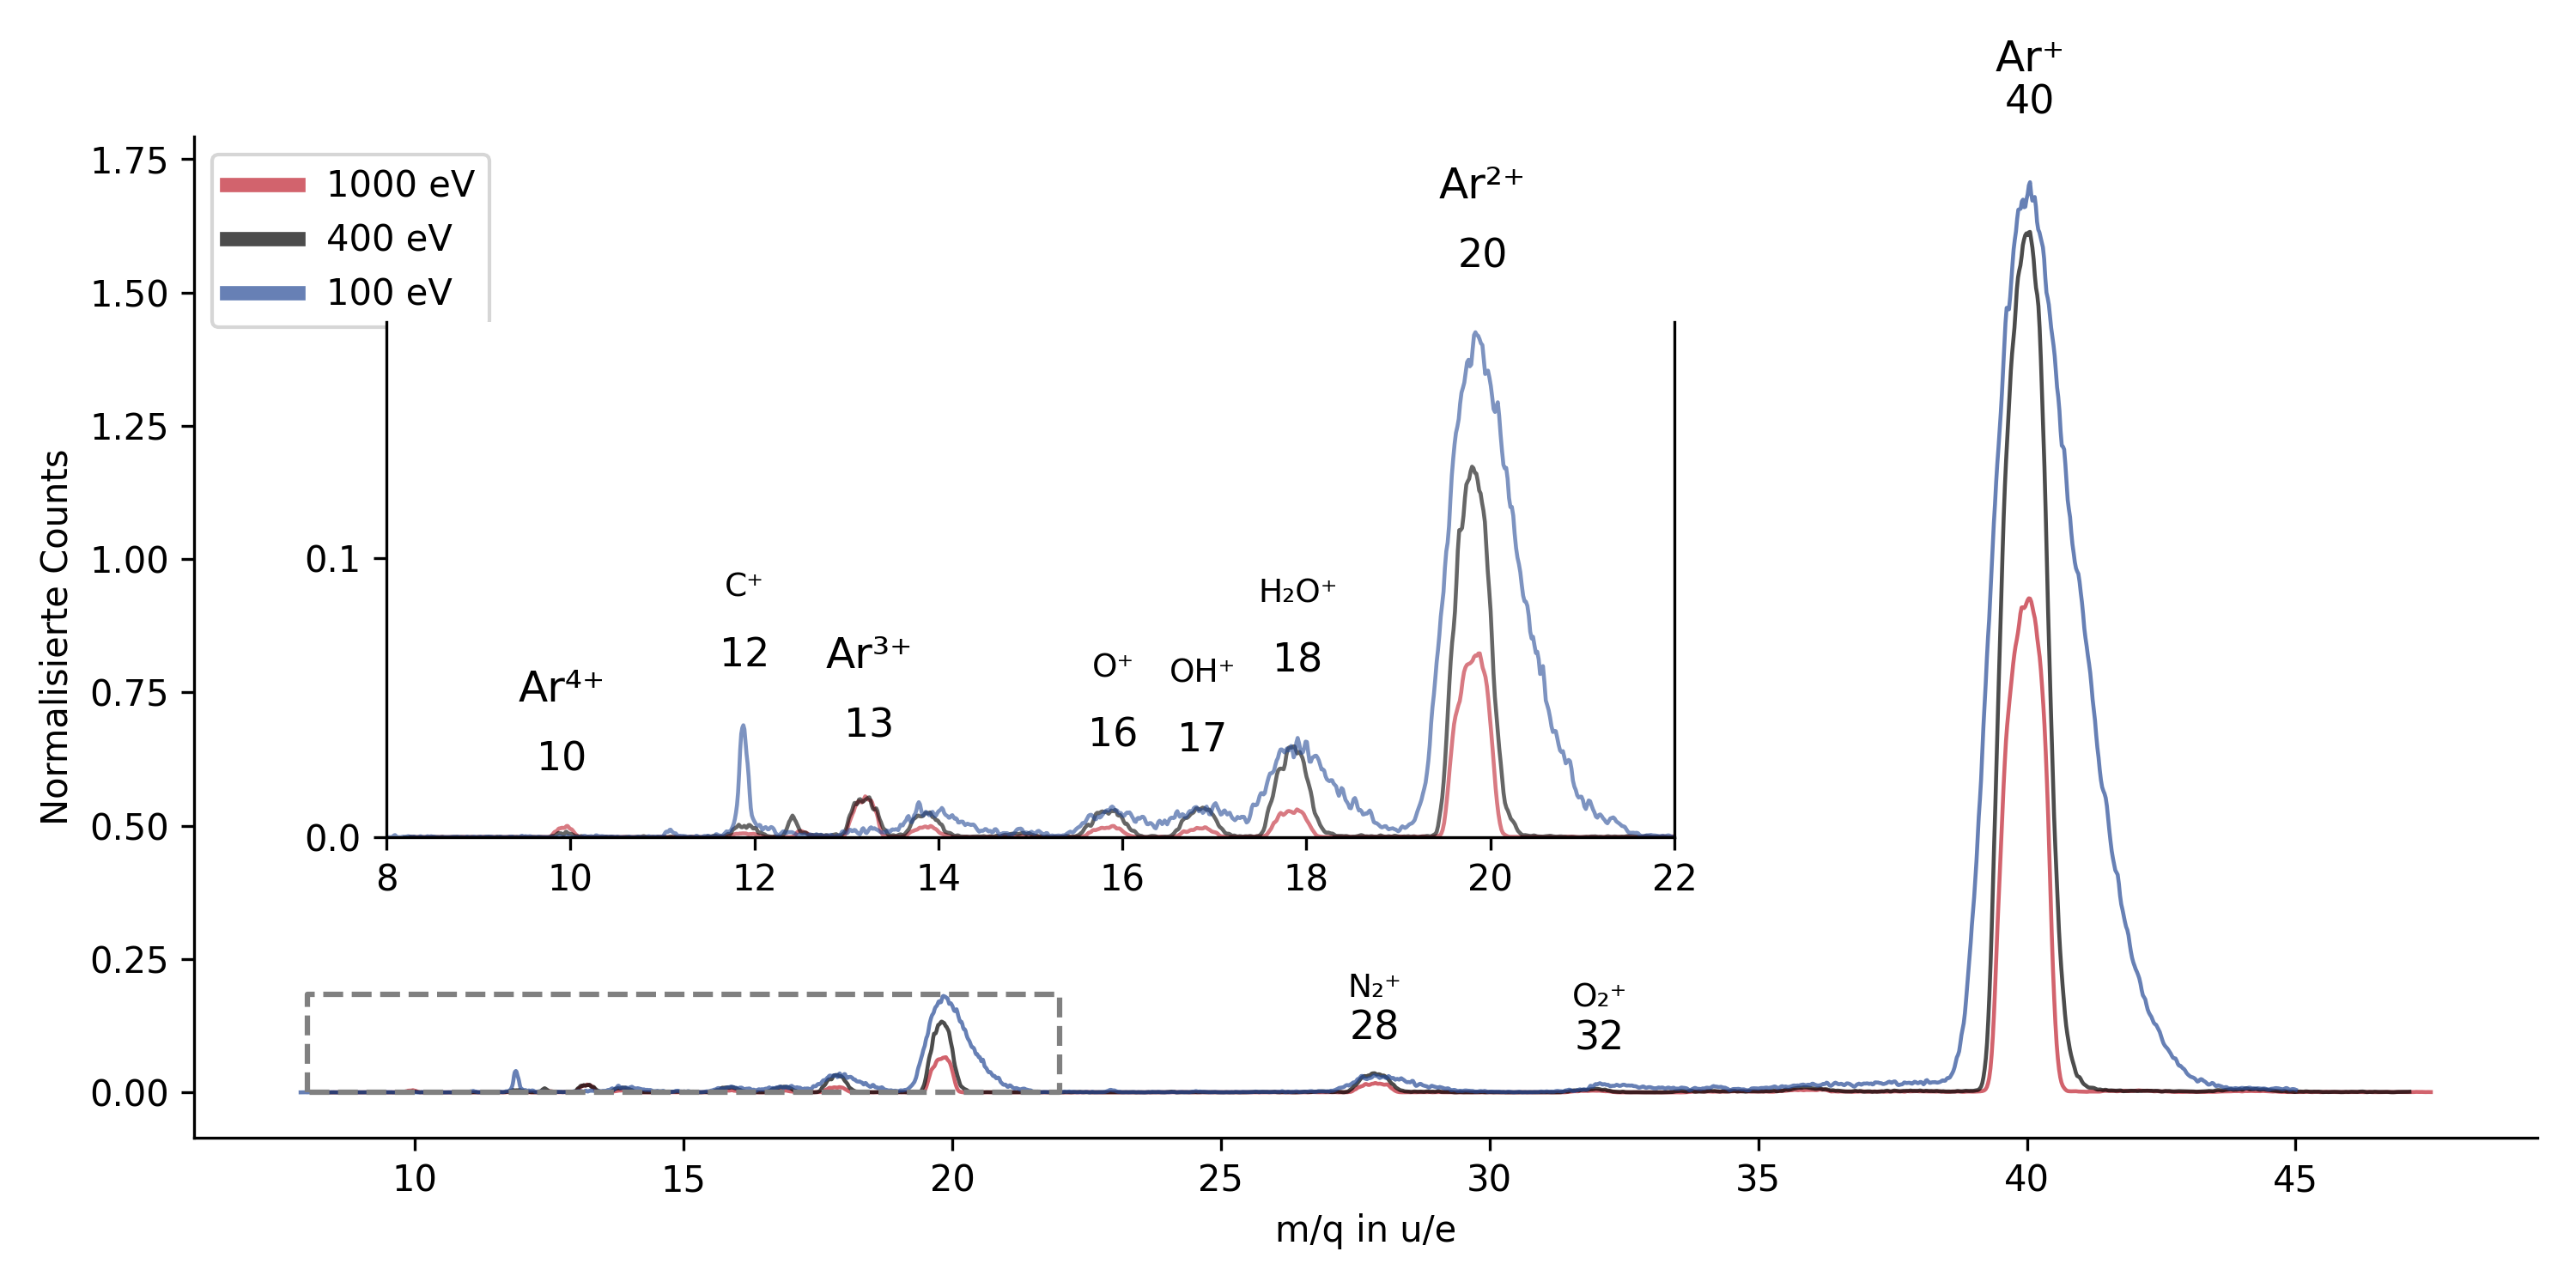
\includegraphics[trim=0 0 0 74, width=1.7\textwidth]{Ar_scaled.png}
            \caption[Skaliertes Massenspektrum von Argon bei verschiedenen Elektronenenergien]{Masse-zu-Ladungsspektrum von Argon bei Elektronenenergien von 100, 400 und 1000 eV. Die Messungen sind jeweils über 30 Minuten entstanden. Die Spektren wurden normalisiert und sind mit den Werten aus \ref{tab:argon} gewichtet dargestellt. Außerdem wurden sie mit einem gaußschen 1D-Filter ($\sigma = 1$) leicht geglättet, um sie besser vergleichen zu können.}
            \label{fig:ar_scaled}
    \end{figure}
\end{landscape}

Obwohl die Werte für die Ionisierungsquerschnitte aufgrund der defekten Kanone nicht direkt ermittelt werden können, soll anhand der relativen Häufigkeiten der Ionen eine qualitative Aussage über die relativen Ionisierungsquerschnitte getroffen werden. 

Der Count der Ionen geht direkt proportional in den Ionisierungsquerschnitt $\sigma_+$ ein. Tabelle \ref{tab:argon} zeigt einen Auszug der Ionisierungsquerschnitte von Argon aus der Arbeit \cite{Straub}. Das bedeutet, dass das Verhältnis der Ionisierungsquerschnitte $\sigma_+$/$\sigma_{2+}$ dem Verhältnis integrierten Counts der entsprechenden Peaks $N_\text{peak}(\text{Ar}^+)$/$N_\text{peak}(\text{Ar}^{2+})$ entsprechen sollte. Abbildung \ref{fig:ar_ratio} zeigt die Grenzen der Integration und die Bestimmung der Verhältnisse. Für einen einfachen Vergleich wurde die Fläche des Ar$^+$-Peaks auf 0.795 normiert, dem entsprechenden Querschnitt aus Tab. \ref{tab:argon}.
Diese Normierung der Fläche des Ar$^{+}$-Peaks auf den Ionisierungsquerschnitt $\sigma_+(E)$ wurde für alle Spektren anhand von Gleichung \ref{eq:norm} durchgeführt und die Ergebnisse in Tabelle \ref{tab:normierte_anzahl} zusammengefasst. Verwendet wird jeweils der Ionisierungsquerschnitt für die entsprechende Elektronenenergie $E$ aus Tabelle \ref{tab:argon}.

\begin{equation}
    \label{eq:norm}
    N_{\text{norm}}(\text{Ar}^{q+}) = N_\text{peak}(\text{Ar}^{q+}) \cdot \frac{\sigma_{+}(E)}{N_\text{peak}(\text{Ar}^{+})}
\end{equation}

Um die Unsicherheit der Ergebnisse abzuschätzen, müssen verschiedene Faktoren berücksichtigt werden. Zunächst ist es wichtig, die Unsicherheit der Masse aufgrund der begrenzten Auflösung des Multi-Channel-Analyzers (MCA) zu betrachten. Diese Auflösung beeinflusst die Breite der Peaks im Massenspektrum. In Abschnitt \ref{sec:transformation} wurde bereits diskutiert, wie diese Unsicherheit entsteht. Die Integrationsgrenzen für die Peak-Fläche wurden, wie in Abbildung \ref{fig:ar_ratio} dargestellt, etwas breiter als die tatsächlichen Peaks gewählt. Dies bedeutet, dass die Unsicherheit in der Peak-Breite nicht wesentlich auf das Ergebnis der Integration einwirkt. Allerdings führt die breitere Wahl der Integrationsgrenzen dazu, dass ein gewisser Teil des Hintergrundrauschens, das auf dem Detektor registriert wird, ebenfalls in die Integration einfließt. Für die Berechnungen wird angenommen, dass dieser Hintergrundrauschen im Vergleich zu den Peaks vernachlässigbar gering ist.

Um die Unsicherheit in der Anzahl der Ionen eines bestimmten Peaks zu bestimmen, sind einige Überlegungen notwendig. Aufgrund der Einzelstoßbedingung können die Stoßionisationen als unabhängige Ereignisse betrachtet werden. Außerdem ist die mittlere Rate der Prozesse bekannt. Deshalb kann die Anzahl der detektierten Ionen als eine Poisson-verteilte Größe angenommen werden. Für eine Poisson-Verteilung ist die statistische Unsicherheit $\sigma_N$ gleich der Quadratwurzel der gesamten Counts im Peak $N_{\text{peak}}(\text{Ar}^{q+})$, die bei Argon mit der Ladung $q$ detektiert wurden. Diese Unsicherheit muss für beide Counts auf der
 
\begin{samepage}
    \begin{table}
        \centering
        \caption[Auszug der Ionisierungsquerschnitte von Argon aus Straub et al.]{Auszug der Ionisierungsquerschnitte von Argon aus Straub et al. \cite{Straub}. Beim Summieren der einzelnen Querschnitte zum totalen Querschnitt werden die Werte entsprechend der Ladung gewichtet:
        $\sigma_{\text{total}} = \sigma_+ + 2\sigma_{2+} + 3\sigma_{3+} + 4\sigma_{4+}$.}
        \label{tab:argon}
        \small
        \begin{tabular}{r c c c c c}
            \toprule
            \textbf{Energie} & $\sigma_+$ & $\sigma_{2+}$ & $\sigma_{3+}$ & $\sigma_{4+}$ & $\sigma_{\text{total}}$ \\
            (eV) & ($10^{-16}$ cm$^2$) & ($10^{-17}$ cm$^2$) & ($10^{-19}$ cm$^2$) & ($10^{-19}$ cm$^2$) & ($10^{-16}$ cm$^2$) \\
            \midrule
            %17  & 0.017  &        &        &        & 0.017  \\
            %20  & 0.46   &        &        &        & 0.46   \\
            %25  & 1.24   &        &        &        & 1.24   \\
            %30  & 1.84   &        &        &        & 1.84   \\
            %35  & 2.26   &        &        &        & 2.26   \\
            %40  & 2.55   &        &        &        & 2.55   \\
            %45  & 2.66   & 0.0048 &        &        & 2.66   \\
            50  & 2.70   & 0.128  &        &        & 2.73   \\
            %55  & 2.69   & 0.418  &        &        & 2.77   \\
            %60  & 2.67   & 0.856  &        &        & 2.84   \\
            %65  & 2.67   & 1.21   &        &        & 2.91   \\
            %70  & 2.67   & 1.46   &        &        & 2.96   \\
            %75  & 2.66   & 1.56   &        &        & 2.97   \\
            %80  & 2.69   & 1.70   &        &        & 3.03   \\
            %85  & 2.70   & 1.79   &        &        & 3.06   \\
            %90  & 2.69   & 1.84   &        &        & 3.06   \\
            %95  & 2.67   & 1.90   & 0.51   &        & 3.05   \\
            100 & 2.64   & 1.89   & 1.03   &        & 3.02   \\
            %110 & 2.61   & 1.91   & 2.21   &        & 3.00   \\
            %120 & 2.55   & 1.87   & 3.23   &        & 2.93   \\
            %140 & 2.45   & 1.77   & 4.94   &        & 2.81   \\
            %160 & 2.35   & 1.65   & 5.57   &        & 2.70   \\
            %180 & 2.27   & 1.58   & 5.68   &        & 2.60   \\
            %200 & 2.18   & 1.44   & 5.53   &        & 2.49   \\
            %225 & 2.10   & 1.31   & 5.30   &        & 2.37   \\
            %250 & 1.99   & 1.25   & 5.23   &        & 2.25   \\
            %275 & 1.87   & 1.13   & 5.09   &        & 2.11   \\
            %300 & 1.79   & 1.08   & 5.03   &        & 2.02   \\
            %350 & 1.63   & 0.953  & 5.99   & 0.17   & 1.84   \\
            400 & 1.51   & 0.872  & 6.32   & 0.44   & 1.71   \\
            %450 & 1.39   & 0.759  & 6.50   & 0.77   & 1.57   \\
            %500 & 1.31   & 0.679  & 6.97   & 1.07   & 1.47   \\
            %550 & 1.23   & 0.623  & 7.08   & 1.18   & 1.38   \\
            %600 & 1.16   & 0.575  & 7.41   & 1.32   & 1.30   \\
            %650 & 1.09   & 0.552  & 7.19   & 1.27   & 1.23   \\
            %700 & 1.03   & 0.524  & 7.23   & 1.33   & 1.16   \\
            %750 & 0.976  & 0.496  & 6.97   & 1.42   & 1.10   \\
            %800 & 0.932  & 0.456  & 6.96   & 1.50   & 1.05   \\
            %850 & 0.901  & 0.425  & 7.09   & 1.42   & 1.01   \\
            %900 & 0.865  & 0.419  & 6.51   & 1.33   & 0.973  \\
            %950 & 0.824  & 0.394  & 6.51   & 1.36   & 0.927  \\
            1000 & 0.795 & 0.374  & 6.57   & 1.32   & 0.895  \\
            \bottomrule
        \end{tabular}
    \end{table}
    
    \begin{table}
        \centering
        \caption[Normierte Anzahl von Ionen]{Normierte Anzahl von Ionen dargestellt wie in Tab. \ref{tab:argon}. Die Unsicherheiten propagieren wie folgt: $\sigma_{\Sigma} = \sqrt{4\sigma_{N_{2+}}^2 + 9\sigma_{N_{3+}}^2 + 16\sigma_{N_{4+}}^2}.
    $}
        \small
        \label{tab:normierte_anzahl}
        \begin{tabular}{llllll}
            \toprule
            \text{} & \multicolumn{5}{c}{\textbf{normierte Anzahl von Ionen}} \\ 
    
            \textbf{Energie} & $N_\text{norm}(\text{Ar}^+)$ & $N_\text{norm}(\text{Ar}^{2+})$ & $N_\text{norm}(\text{Ar}^{3+})$ & $N_\text{norm}(\text{Ar}^{4+})$ & gew. Summe \\
            (eV) & (1) & ($10^{-1}$) & ($10^{-3}$) & ($10^{-3}$) & ($1$) \\
            \midrule
            50  & {2.7}  & {0.206 $\pm$ 27e-2} & {}  & {}  & {2.41 $\pm$ 54e-3}   \\
            100 & 2.64  & 1.42 $\pm$ 69e-2 & 4.04 $\pm$ 12 & {} & 2.94 $\pm$ 14e-2 \\
            400 & 1.51  & 0.602 $\pm$ 46e-2 & 4.62 $\pm$ 13 & 0 $\pm$ 0 & 1.64 $\pm$ 99e-3 \\
            1000 & 0.795  & 0.278 $\pm$ 31e-2 & 3.98 $\pm$ 12 & 0.763 $\pm$ 5 & 0.86 $\pm$ 74e-3 \\
            \bottomrule
        \end{tabular}
    \end{table}
    
    \begin{table}
        \centering
        \caption[Prozentuale Abweichungen zu Straub et al.]{Prozentuale Abweichungen der normierten Anzahl von Ionen zu den Werten von Straub et al. \cite{Straub}.}
        \small
        \label{tab:abweichungen}
        \begin{tabular}{llllll}
            \toprule
            \text{} & \multicolumn{5}{c}{\textbf{prozentuale Abweichungen}} \\ 
    
            \textbf{Energie} & $N_\text{Ar}^+$ & $N_\text{Ar}^{2+}$ & $N_\text{Ar}^{3+}$ & $N_\text{Ar}^{4+}$ & gew. Summe \\
            (eV) & (1) & ($10^{-1}$) & ($10^{-3}$) & ($10^{-3}$) & ($1$) \\
            \midrule
            50  & {}  & {60.9\ \%} & {}  & {}  & {11.7\ \%}   \\
            100 & {}  & 24.9\ \% & 292.2\ \% & {} & 2.6\ \% \\
            400 & {}  & 31.0\ \% & 26.9\ \% & 100\ \% & 4.1\ \% \\
            1000 & {}  & 25.7\ \% & 39.4\ \% & 42.2\ \% & 3.9\ \% \\
            \bottomrule
        \end{tabular}
    \end{table}
\end{samepage}

\begin{figure}
    \hspace{-1.1cm}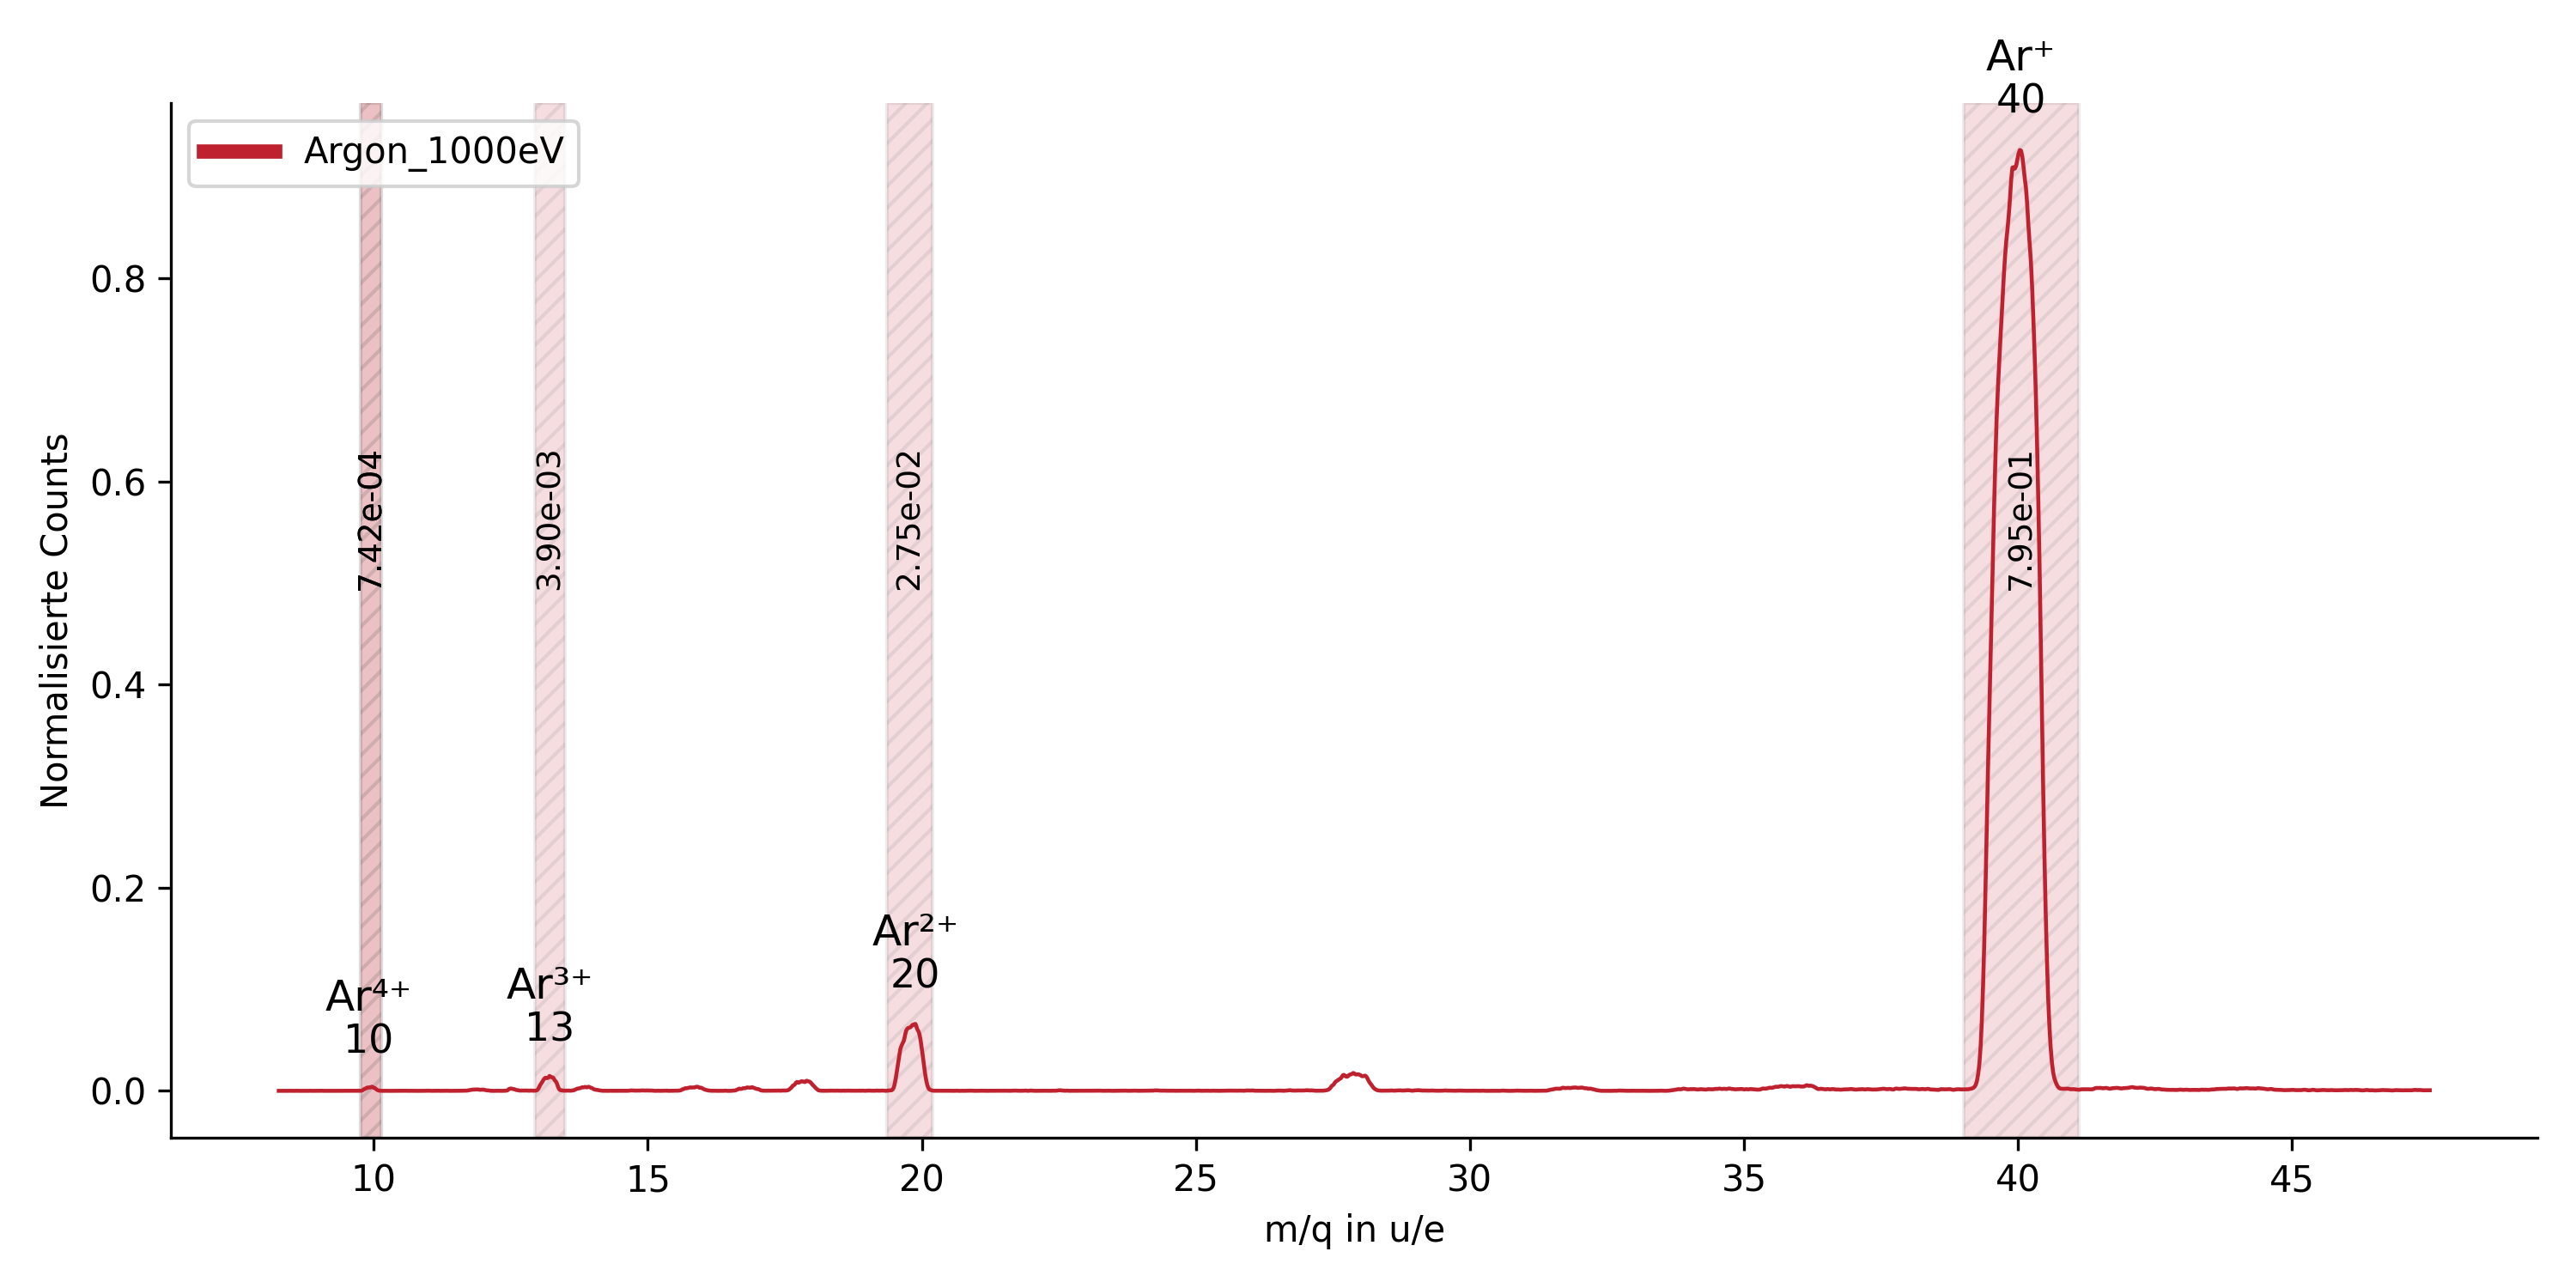
\includegraphics[width=1.08\textwidth]{Ar_integrated.png}
    \caption[Integration eines, auf die Werte von Straub et al. gewichteten, Argonspektrums bei 1000 eV]{Integration eines gewichteten Argonspektrums bei 1000 eV.}
    \label{fig:ar_ratio}
\end{figure}

rechten Seite von Gleichung \ref{eq:norm} berücksichtigt werden.

Ein weiterer wichtiger Aspekt ist die Unsicherheit, die aus der Normierung auf den Ionisierungsquerschnitt von Straub et al. resultiert. Der Ionisierungsquerschnitt $\sigma_+(E)$ wurde mit einer Unsicherheit von $\pm 3.5$ \% für alle verwendeten Elektronenenergien $E$ angegeben. Diese Unsicherheit propagiert dann auch in die normierten Werte der Ionenzahlen. 

Die Gesamtunsicherheit der relativen Häufigkeiten der Ionen kann dann durch die quadratische Addition der Unsicherheitsquellen berechnet werden. Die Umformung der Fehlerfortpflanzung und die Gleichung für die Unsicherheit der normierten Ionenzahl $\sigma_\text{peak, norm}$ ist aufgrund ihrer Länge im Anhang \ref{sec:fehlerfortpflanzung} zu finden.

In Tabelle \ref{tab:normierte_anzahl} sind neben den normierten Werte der Ionen auch ihren Unsicherheiten dargestellt. Tabelle \ref{tab:abweichungen} gibt die prozentualen Abweichungen zu den Werten von Straub et al. \cite{Straub} an. Es ist zu erkennen, dass die Werte für die ein- und zweifach geladenen Ionen besser übereinstimmen, während die Werte für die dreifach und vierfach geladenen Ionen größere prozentuale Abweichungen haben. Abbildung \ref{fig:uncertainties} zeigt den relativen Vergleich der Verläufe der normierten Ionenanzahlen mit den Unsicherheiten über der Elektronenenergie von Straub et al. und dieser Arbeit. Im Energiebereich ab 100 eV haben die Werte eine gute Übereinstimmung. Bei niedrigeren Energien sind die Unsicherheiten jedoch deutlich größer. Die Abweichung bei geringen Energien könnte auch von der beschädigten Elektronenkanone beeinflusst sein und muss in späteren Experimenten überprüft werden. Insgesamt zeigt die qualitative Auswertung allerdings, dass die Anlage erfolgreich arbeitet, da die relativen Häufigkeiten der Ionen den Erwartungen allgemein gut entsprechen.  


\begin{figure}
    \centering
    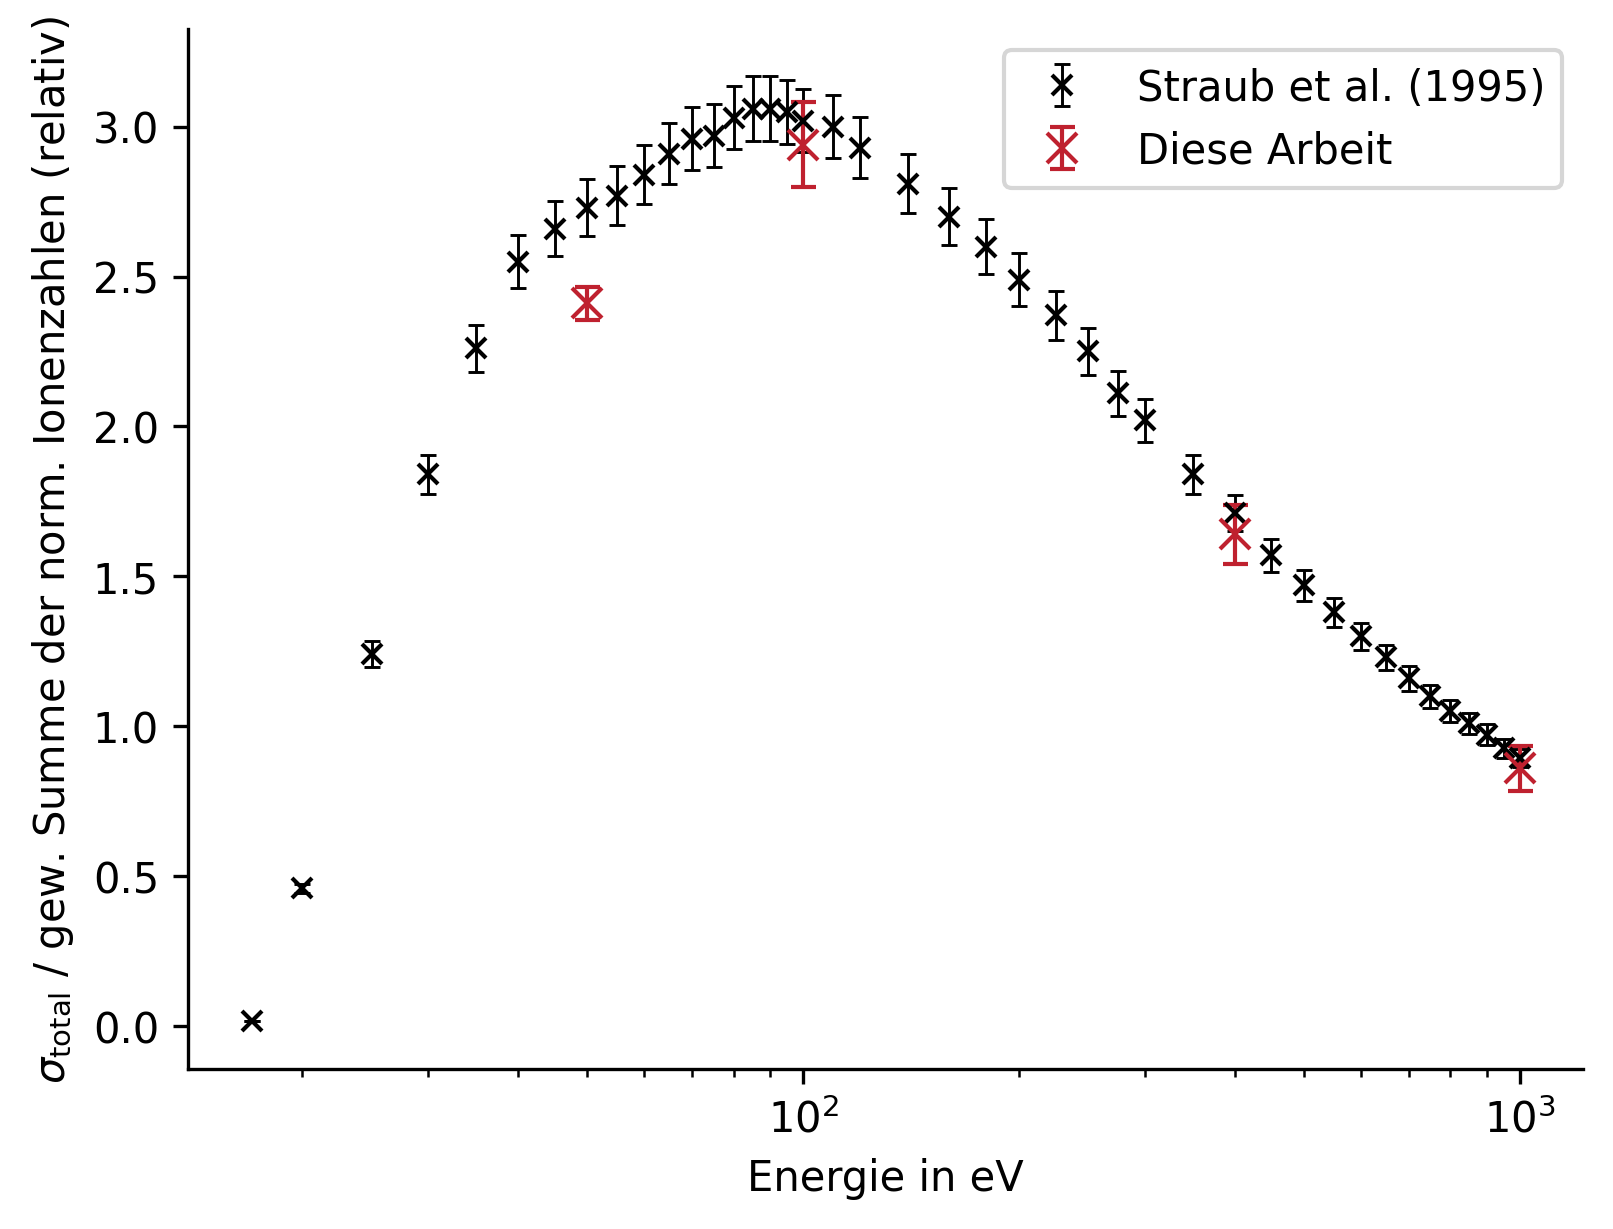
\includegraphics[width=.85\textwidth]{uncertainties.png}
    \caption[Relativer Vergleich des totalen Ionisierungsquerschnitts mit Straub et al.]{Relativer Vergleich des totale Ionisierungsquerschnitts $\sigma_\text{total}(E)$ über der Elektronenenergie zu den Werten von Straub et al. \cite{Straub} mit entsprechender Unsicherheit.}
    \label{fig:uncertainties}
\end{figure}

\section{Restgasspektrum}
\label{sec:Restgasspektrum}
Eine weitere Möglichkeit zur Überprüfung des Massenspektrometers ist die Aufnahme eines Restgasspektrums. Hierbei wird kein Gas in die Kammer eingelassen und lediglich der atmosphärische Hintergrund in der Kammer gemessen. Dieser besteht aus verschiedenen Restgasen, die durch die Elektronenstoßionisation genauso ionisiert werden können. In einem Vakuum erwartet man vor allem Rückstände von Wassermolekülen sowie stabiler Kohlenstoffverbindungen, die bei der Vakuumbildung aus den Wänden der Kammer gelöst werden, als auch Reste von Stickstoff und Sauerstoff aus der Luft. Außerdem können besonders leichte Gase, hier vor allem Wasserstoff, übrig bleiben, da sie besonders flüchtig sind und die Vakuumpumpen sie weniger effektiv entfernen können. Es ist zusätzlich praktisch die Restgasverteilung zu kennen, um sie bei der Auswertung von Messungen berücksichtigen zu können. Aufgrund der geringen Dichte und damit niedrigem Ionisierungsquerschnitt muss diese Messung lange durchgeführt werden. 

Wie bereits bei der Kalibrationsmessung muss das Massenspektrum transformiert werden, um die Masse-zu-Ladungsverhältnisse der Ionen zu bestimmen. Dafür wird für einige der Peaks anhand von den Erwartungen eine Annahme getroffen, welchem Verhältnis sie entsprechen könnten. Für die Identifikation der Ionen wurde angenommen, das der größte Peak ionisierten Wassermolekülen
entspricht und der erste Peak ionisiertem Wasserstoff. Das resultierende, skalierte Restgasspektrum ist in Abb. \ref{fig:rest} dargestellt.

Wie erwartet, können die größten Peaks auf ionisierte Wassermoleküle sowie Wasserstoff zurückgeführt werden. Auch die Peaks von molekularem Stickstoff, Sauerstoff und vermutlich Kohlenstoffdioxid sind gut zu erkennen. Die Struktur und Übereinstimmung des Restgasspektrums bestätigen, dass die Anlage korrekt funktioniert und zur Identifikation von Produktionen verschiedener Massen und Ladungen nutzbar ist. Außerdem ist zu erkennen, dass Massendifferenzen von 1 $u$ im Bereich leichter Ionen aufgelöst werden können. 

\begin{figure}
    \hspace{-1.1cm}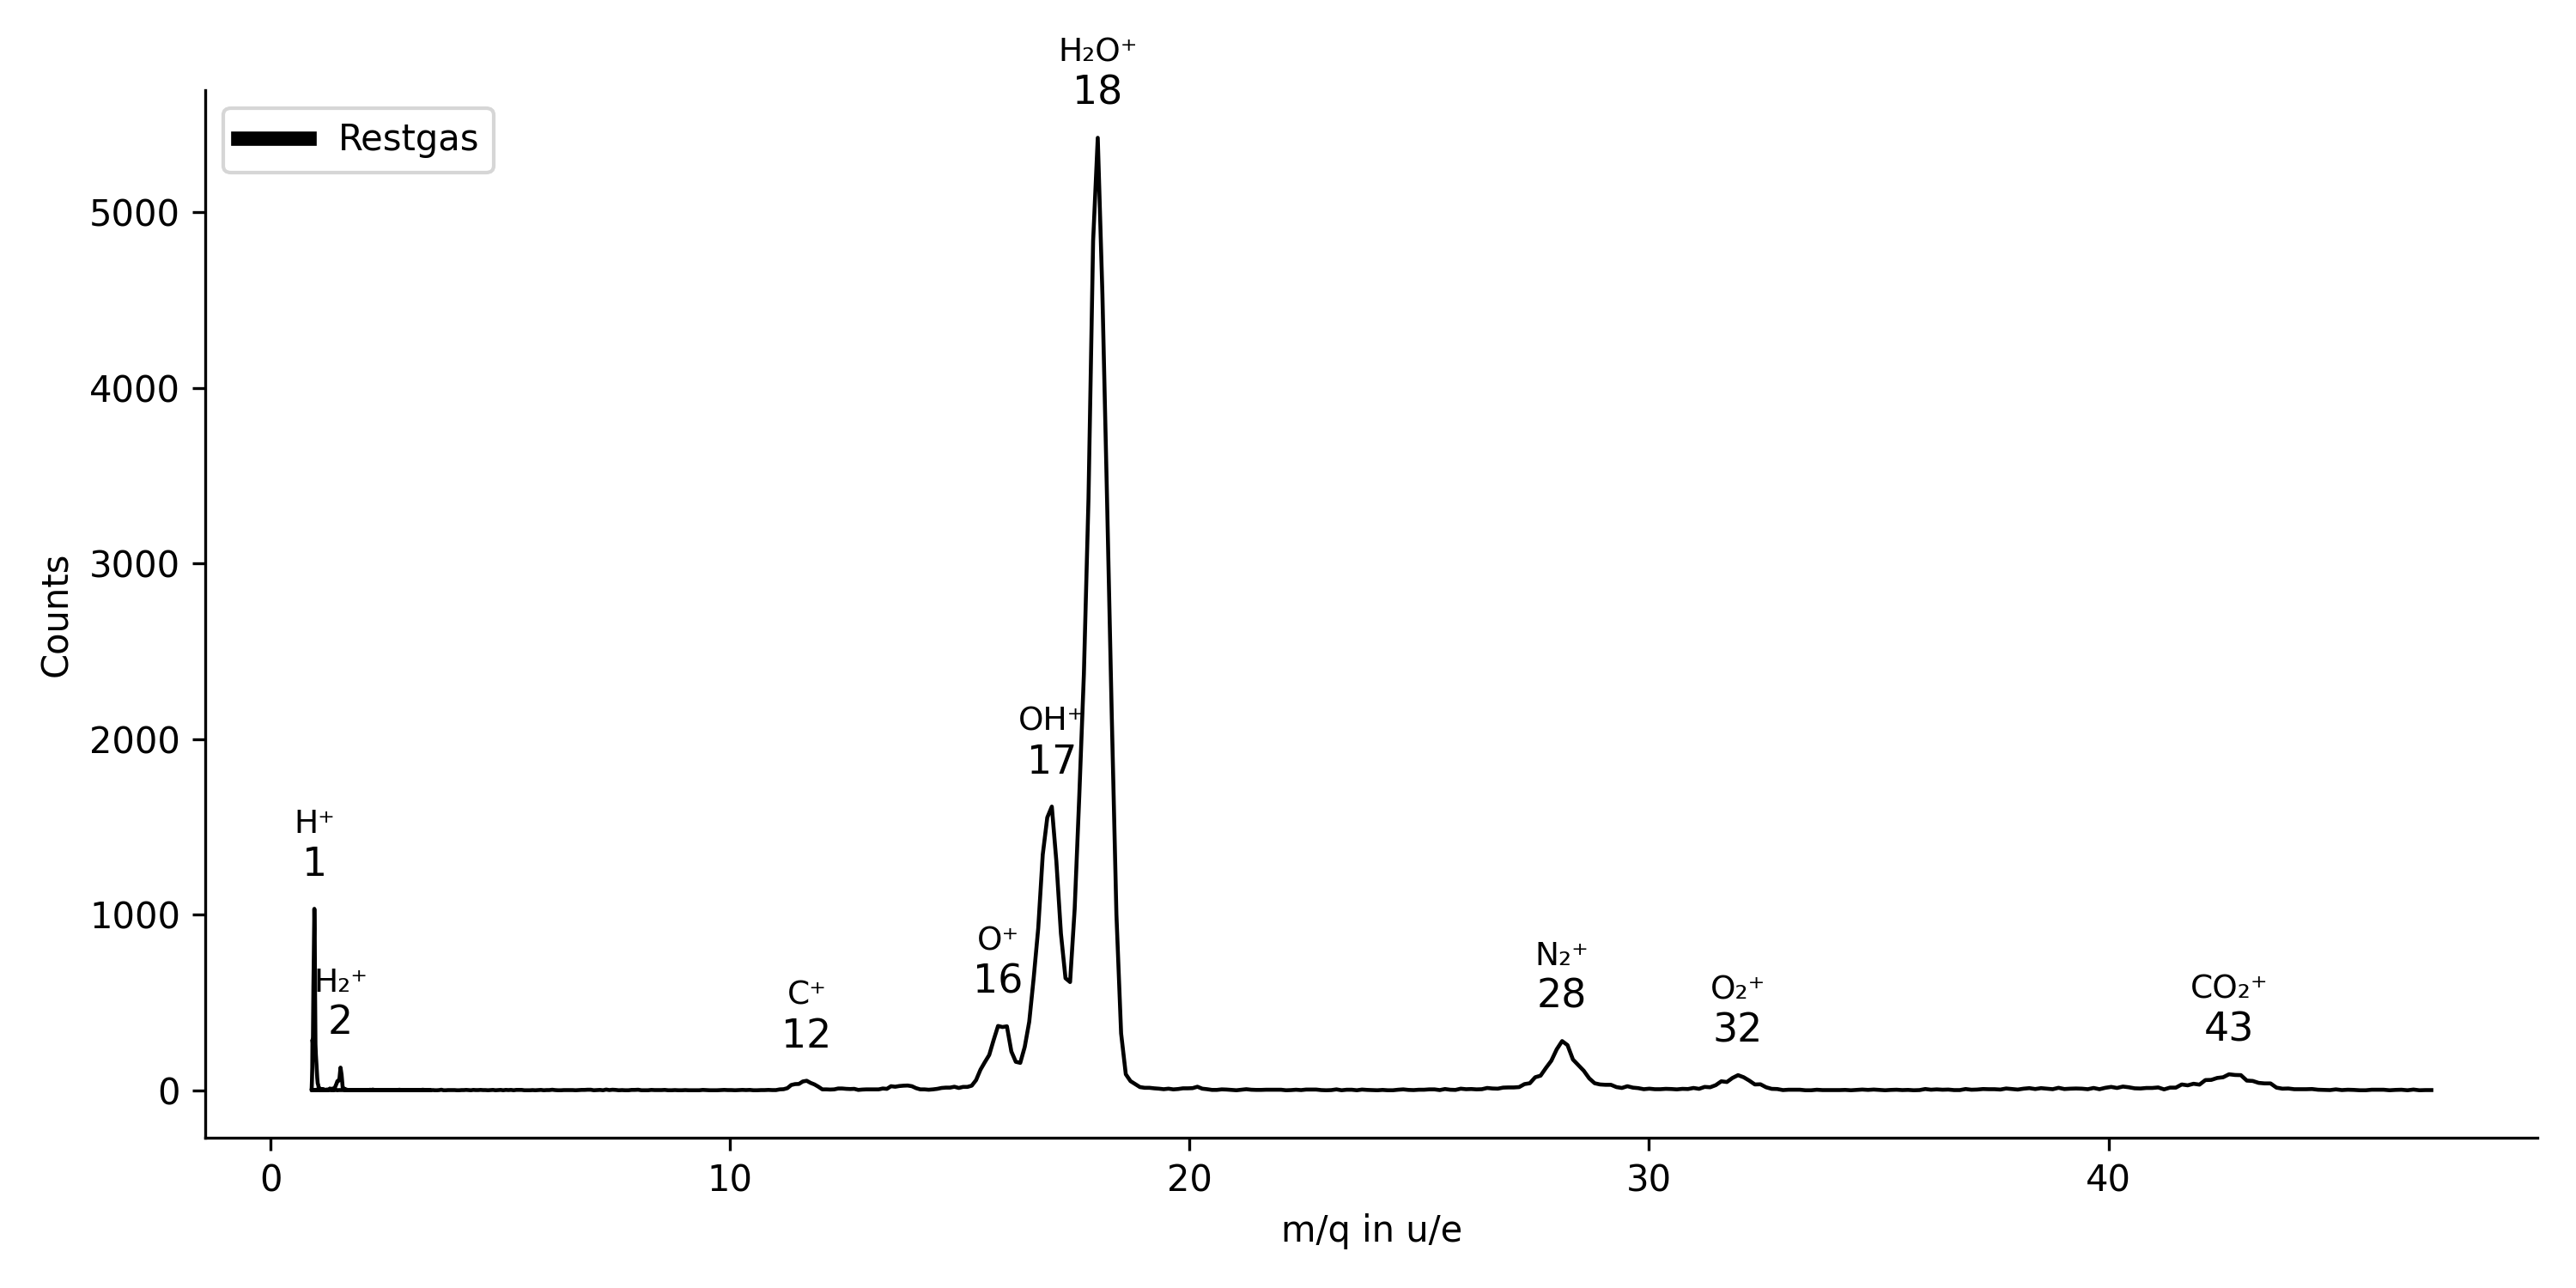
\includegraphics[width=1.08\textwidth]{Restgas.png}
    \caption[Masse-zu-Ladungsspektrum der Restgase]{Masse-zu-Ladungsspektrum der Restgase nach Transformation aus einem Flugzeitspektrum. Die Messung ist über mehrere Stunden entstanden.}
    \label{fig:rest}
\end{figure}

\section{Auswertung der Positionsdaten}
Anhand der vom Detektor aufgenommenen Positionsdaten der Ionen können Rückschlüsse auf den Entstehungsort der Ionen gezogen werden. Abbildung \ref{fig:Strahl} zeigt einen Plot dieser Daten für eine Messung mit Argonionen. Es ist zu erkennen, dass die Ionen, wie erwartet, entlang eines horizontalen Streifens entstehen, der seitlich abgeschnitten ist. Die Ionen wurden durch das 2 cm große Loch in der Deckenplatte des Beschleunigungskondensators auf den Detektor geschossen. Deshalb ist das Abbild des Elektronenstrahls seitlich begrenzt. Die Entstehungsorte der Ionen sind offensichtlich stark mit dem Strahl korreliert, was zeigt, dass die Ionen entlang des Strahls entstehen und nicht wesentlich abgelenkt werden oder aus anderen Quellen stammen.

\subsection{Anomalien}
\label{sec:Anomalien}
\begin{figure}
    \hspace{-1.1cm}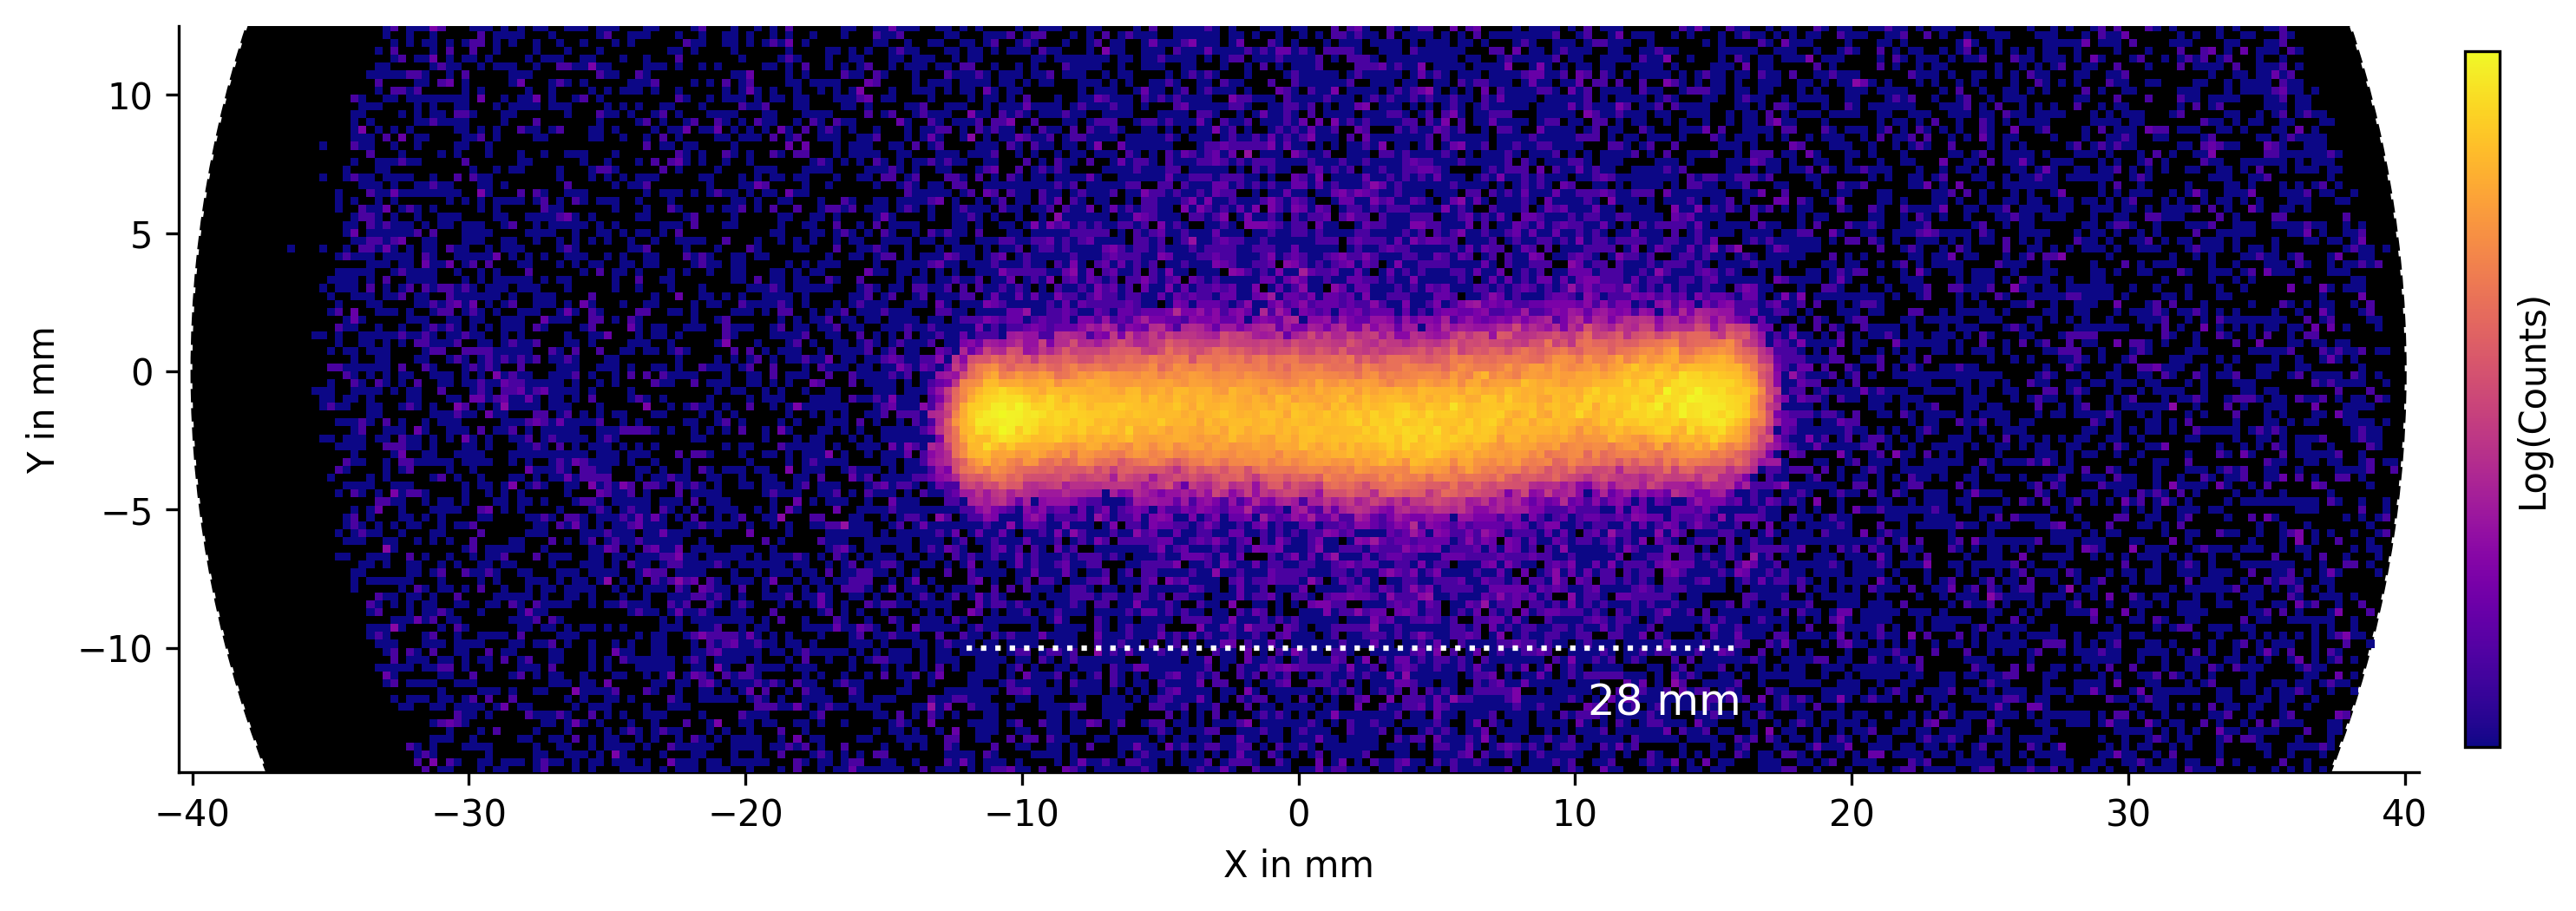
\includegraphics[width=1.08\textwidth]{Strahl.png}
    \caption[Logarithmisches Abbild des Strahls auf dem Detektor]{Positionsbestimmung der detektierten Teilchen auf dem Detektor zeigt den Strahl bei einer Elektronenenergie 100 eV auf dem Detektor. Die Anzahl der Treffer in einem Pixel wird logarithmisch skaliert von den Farben angegeben. Da der Detektor schief verbaut ist, wurde das Bild im Nachhinein gedreht. Das Abbild des Strahls ist seitlich begrenzt, da die Ionen durch das 2 cm große Loch in der Deckenplatte auf den Detektor gelangen. Die geometrische Größe des Detektors ist in Schwarz eingezeichnet.}
    \label{fig:Strahl} 
\end{figure}
Auffällig sind jedoch die Überhöhungen an den seitlichen Rändern des Strahls, die in Abbildung \ref{fig:Strahl3D}, einer absoluten Darstellung der Counts als 3D-Plot, besonders deutlich zu erkennen sind. Außerdem ist die Länge des Abbilds von 28 mm unvorhergesehen. Bei geraden Flugbahnen der Ionen würde ein Abbild von etwa 20 mm Länge erwartet werden, entsprechend dem Loch in der Deckenplatte. Anders als bei einem Ionenstrahl, bei dem die Coloumbabstoßung eine Aufweitung bewirkt, sollte kein solcher Effekt unter der Einzelstoßbedingung auftreten. Dennoch ist es statistisch möglich, dass mehrere Ionen gleichzeitig extrahiert werden, auch wenn es im Mittel nur ein Ion ist. Das könnte für die Verbreiterung des Strahls und für die Erhöhung an den Seiten verantwortlich sein. Außerdem kann die thermische Bewegung der Gasteilchen das Abbild des Strahls verschwimmen lassen, sodass dieser breiter erscheint. Beide dieser Effekte sollen mit einer Simulation der Ionenoptik in Kapitel \ref{sec:annomalies_sim} überprüft werden. Die leichte Wölbung des Strahls war während des Experiments konstant und kann nur auf eine Ungenauigkeit der vom Detektor ermittelten Positionen zurückgeführt werden. 

\begin{figure}
    \hspace*{-0cm}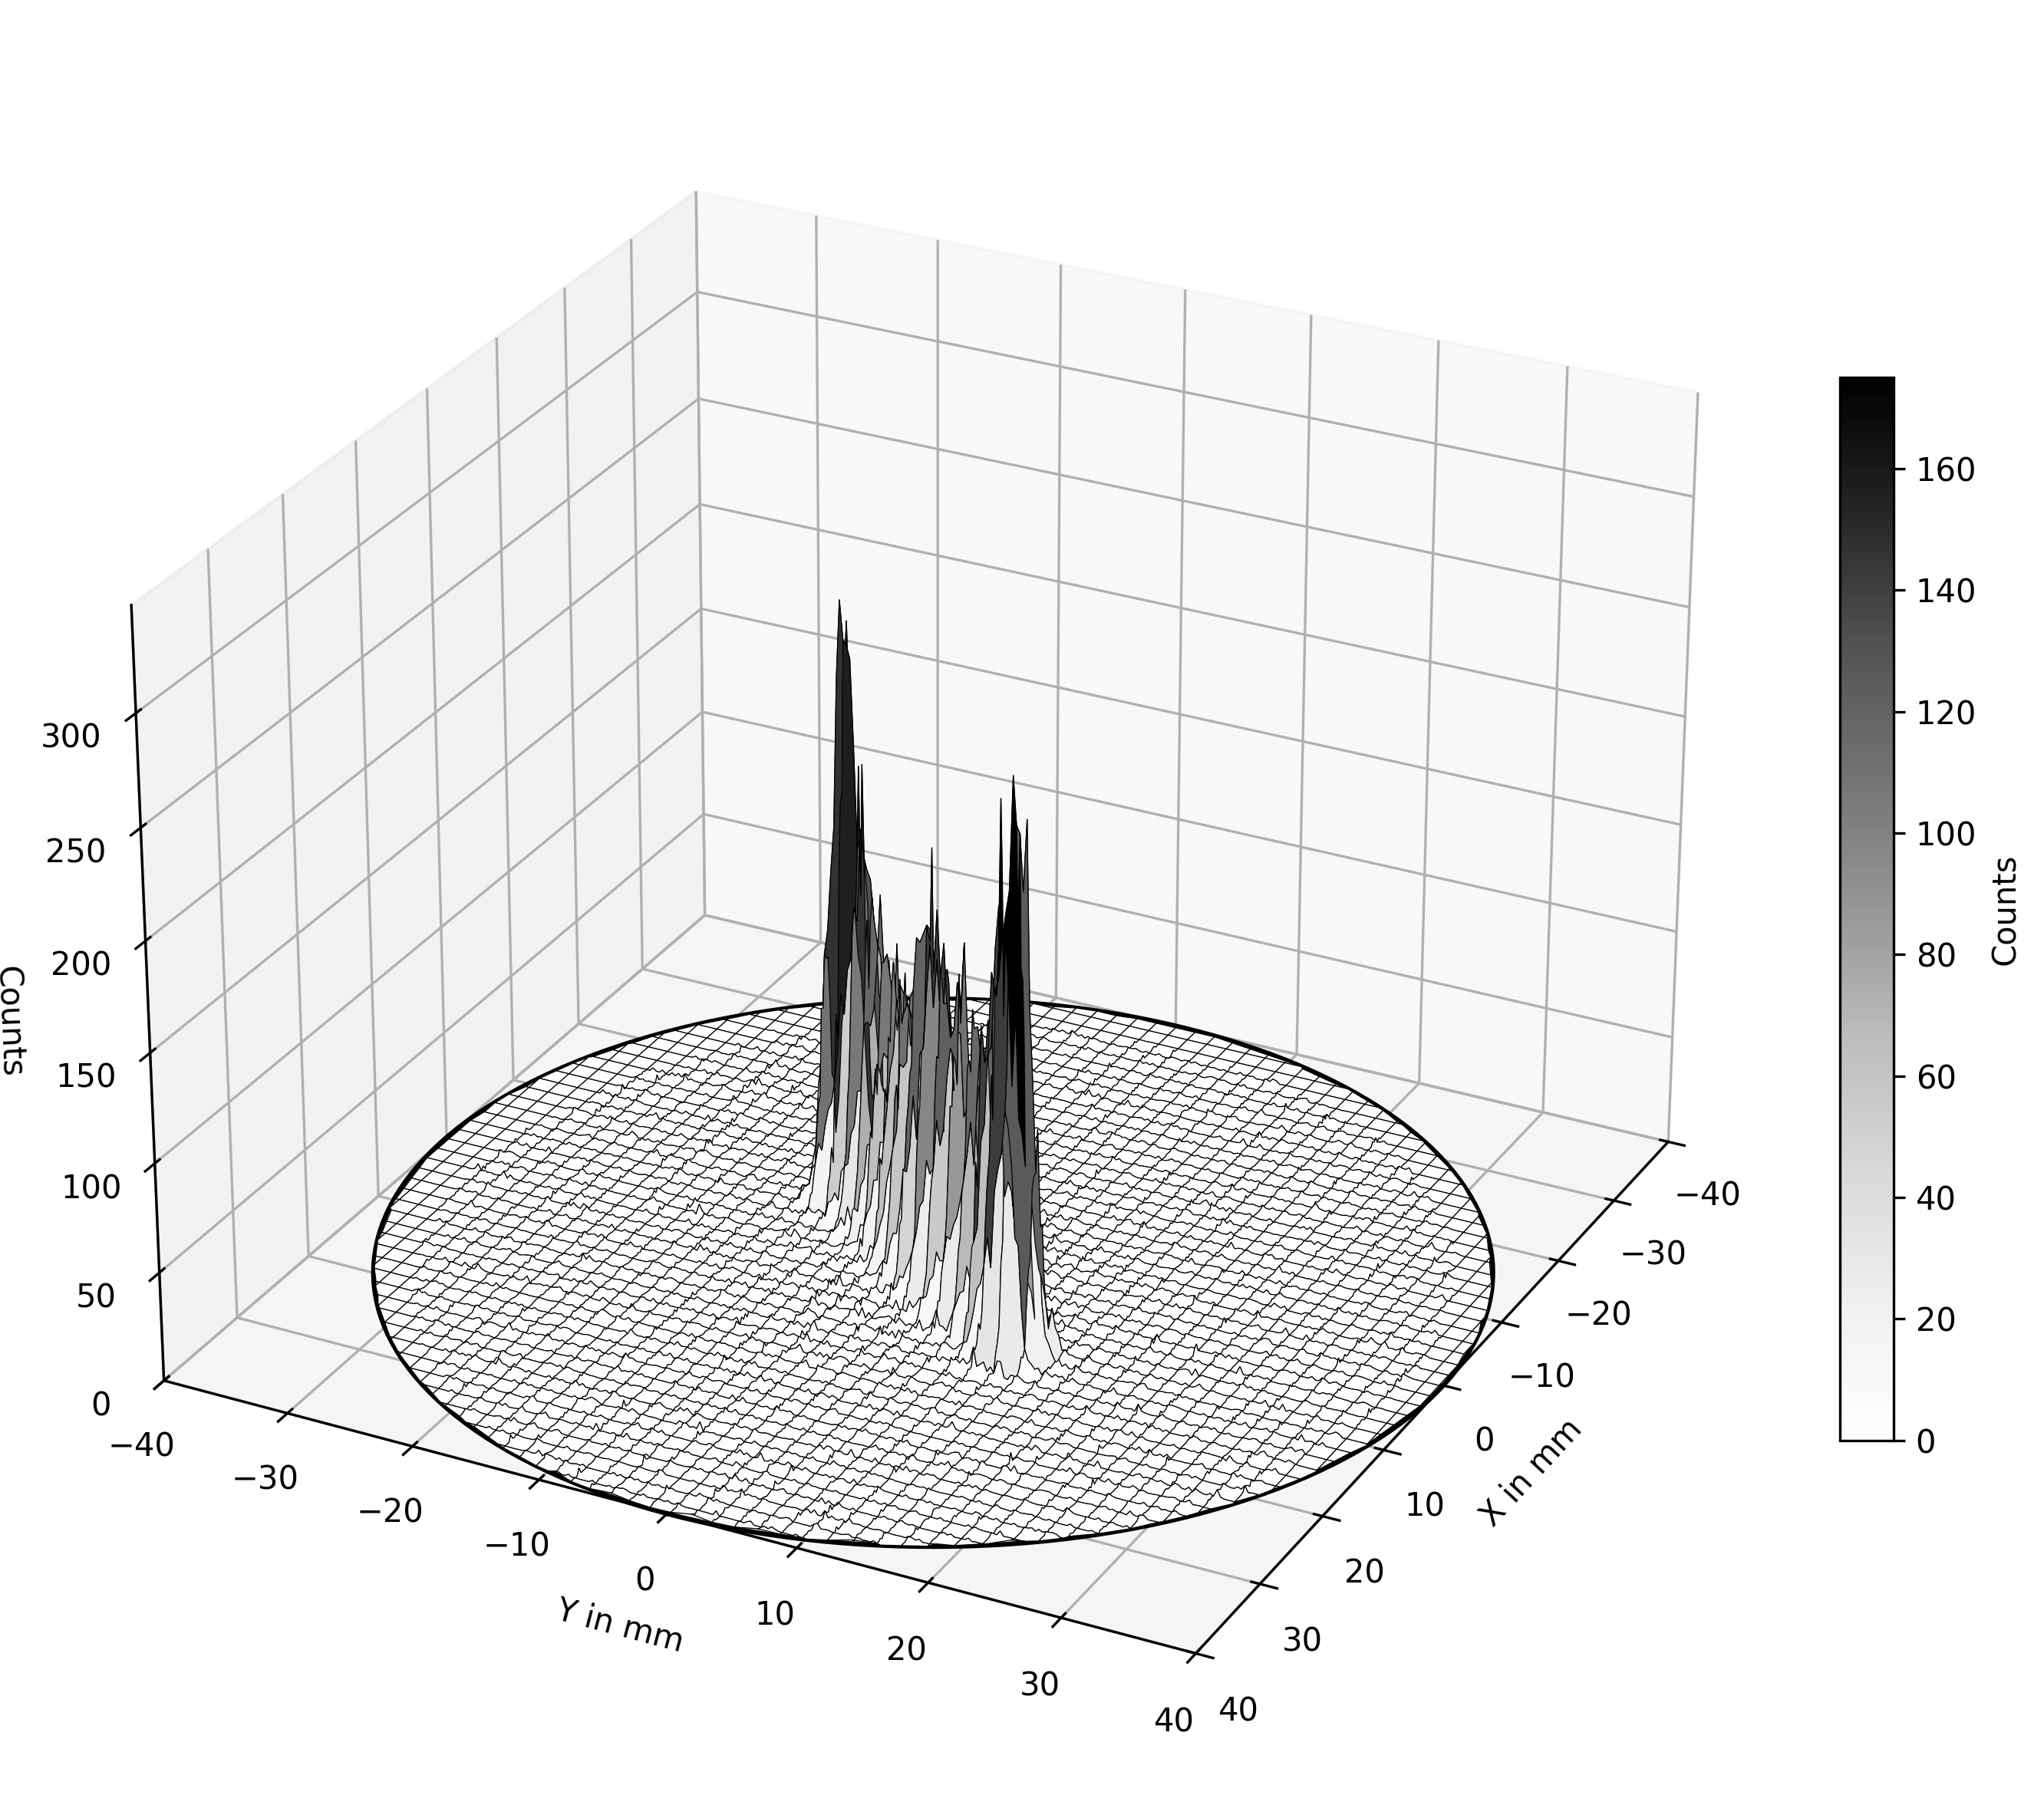
\includegraphics[width=1\textwidth]{Strahl3D.png}
    \caption[Dreidimensionale Darstellung des Strahls auf dem Detektor]{Dreidimensionale Darstellung des Strahls auf dem Detektor. Die z-Achse gibt die absoluten Counts an. Die Überhöhungen an den Rändern des Strahls sind gut zu erkennbar. Das Bild zeigt die tatsächliche Ausrichtung des Detektors relativ zum Strahl.}
    \label{fig:Strahl3D} 
\end{figure}

\subsection{Ermittlung des Elektronenstrahlprofils}
\label{sec:profil}
Die Positionen der detektierten Ionen auf dem Detektor können genutzt werden, um das Strahlprofil, also die räumliche Verteilung der Teilchen in einem Schnitt des Strahls, zu bestimmen. Um das Strahlprofil über die ganze abgebildete Länge zu mitteln, wird Daten-Binning genutzt. Das bedeutet, dass für jede y-Koordinate in einem Bin die Counts aller detektierten Ionen aufsummiert werden. Das Ergebnis ist ein Histogramm, das die räumliche Verteilung der Elektronen entlang der y-Achse zeigt. Es ist in Abb. \ref{fig:Strahlprofil} dargestellt. Für das Profil des Strahls wird eine Gauß-Verteilung erwartet, da thermische Effekte und Beugung die Position der Elektronen zufällig beeinflussen. Mit einem Fit der Daten mit einer Gauß-Funktion kann die Breite des Strahls bestimmt werden. In der Abbildung ist zu erkennen, dass die Abweichung der Daten vom Fit sehr klein ist. Über die Parameter der gefitteten Funktion kann die volle Breite bei halbem Maximum (FWHM) des Strahls bestimmt werden. Sie beträgt 2.93 mm bei 100 eV. Obwohl diese Strahlbreite in die vom Hersteller angegebene Fleckgröße von 5 mm passt, ist sie wahrscheinlich, ähnlich wie die horizontale Länge des Strahls, tatsächlich kleiner als ihr Abbild, das hier ausgewertet wurde. Wenn man annimmt, dass die Vergrößerung entlang der y-Achse ähnlich der entlang der x-Achse ist, sollte der Strahl eine FWHM von etwa 2 mm aufweisen.

\begin{figure}
    \centering
    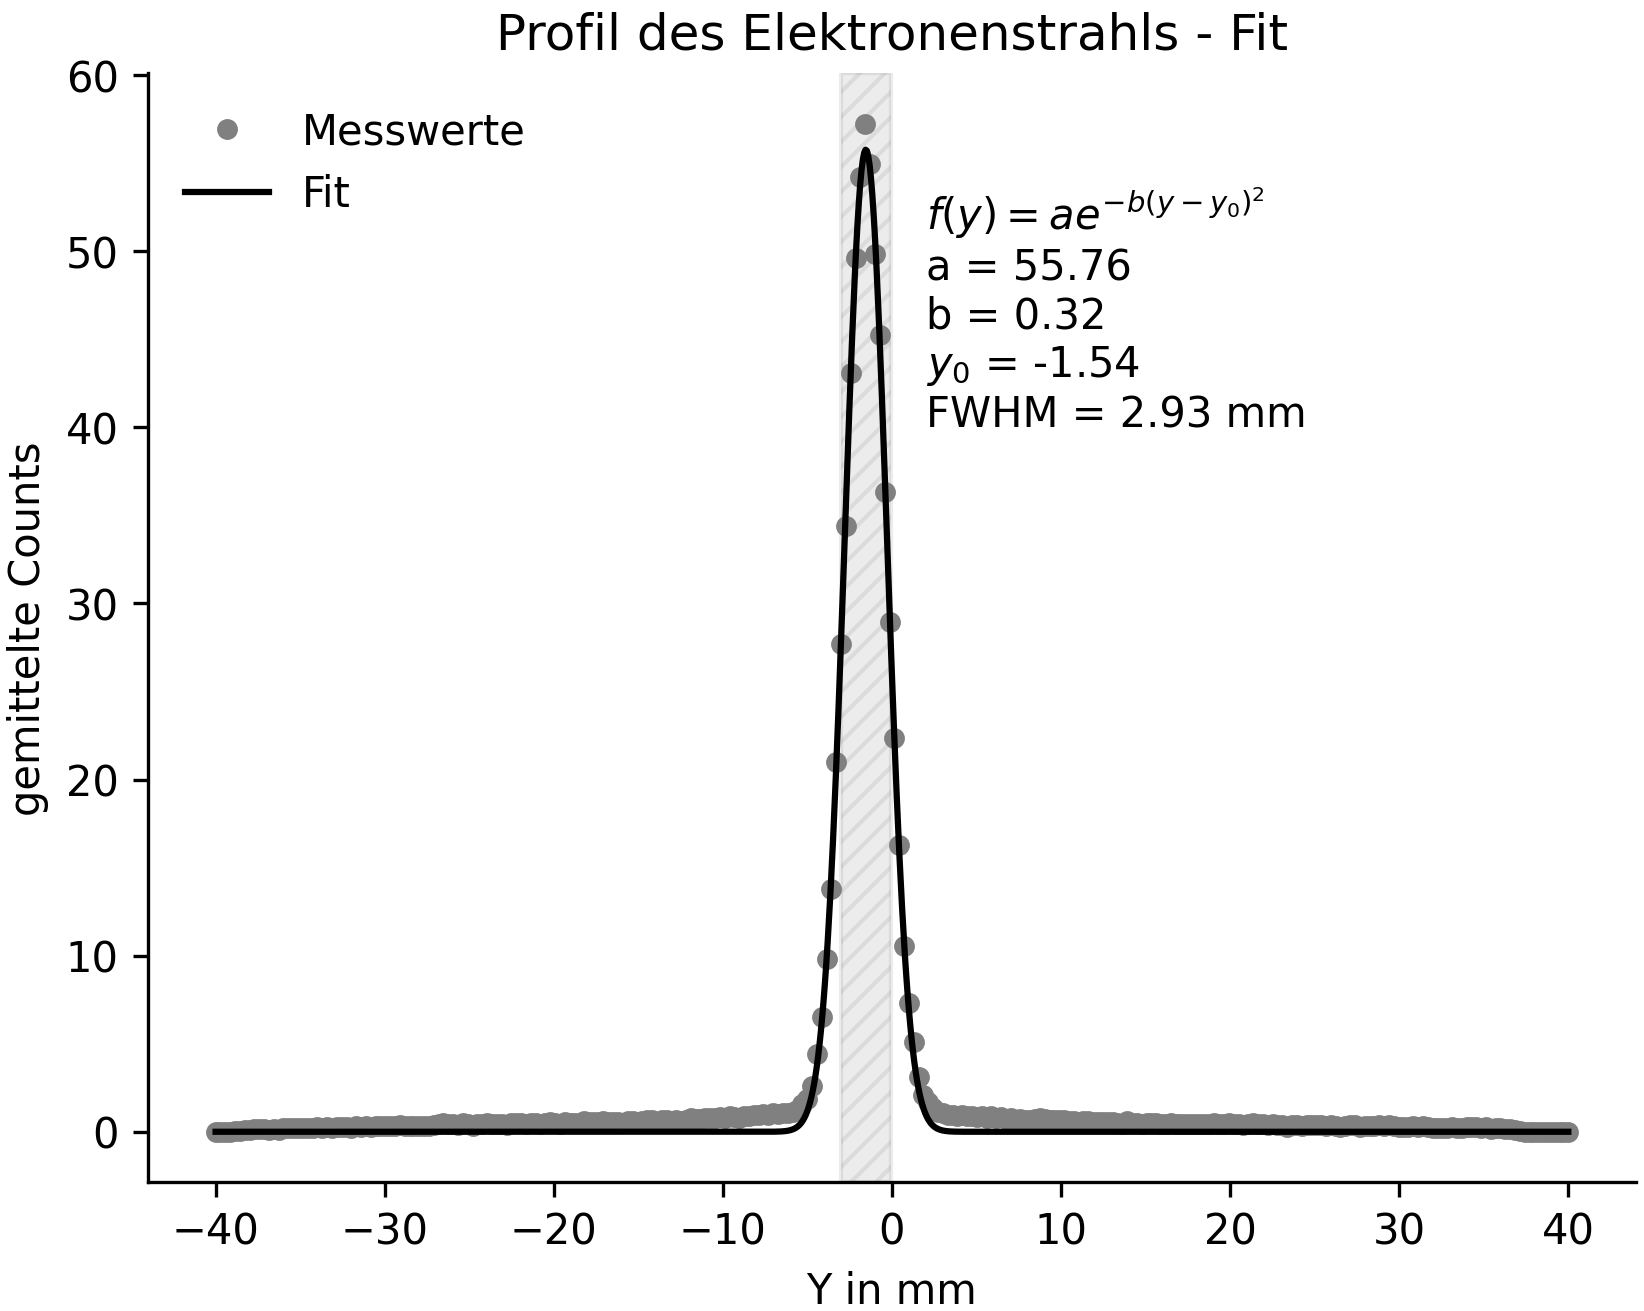
\includegraphics[width=.9\textwidth]{Strahlprofil.png}
    \caption[Gemitteltes Strahlprofil]{Gemitteltes Strahlprofil aus den Positionen der detektierten Ionen. Die Daten wurden mit einem Gaußfit gefittet, um die Breite des Strahls zu bestimmen. In grau-schraffiert eingezeichnet ist die volle Breite bei halbem Maximum (FWHM) des Strahls abgebildet.}
    \label{fig:Strahlprofil} 
\end{figure}